%!TEX root = ../thesis.tex
\chapter{The Pleiades as a benchmark}
\label{chap:pleiades}

\section{Generalities}
The ancient greeks named Pleiades to a crowded group of nine stars which they believe share a common origin. These stars were the seven sisters, that together with their parents the titan Atlas and the nymph Pleione, were put in the sky  by the god Zeus.
 
Today, we call the Pleiades cluster not just to the nine stars that made up the original Pleione family, but to a much larger group, which according to \citet{Bouy2015} adds up to $\sim2100$ members. This cluster is fairly close to the sun, $\sim 136\,pc$ \cite[according to][]{Galli2017}, and is also young in galactic scales, with only $\sim125\,Myr$ \citep{Stauffer1998}. Since it is located in the solar neighbourhood it has a distinctive angular velocity in the plane of the sky: about $-16\,mas/yr$ in right ascension and $20\,mas/yr$ in declination. Also, it has expelled most of its cocoon gas, which gives it an almost null extinction of $A_v=0.12$ \citep{Guthrie1987}. These properties make the Pleiades one of the most studied cluster in the history of astronomy \footnote{Probably just after Orion.}. Thus making it also the perfect test case of the methodology developed in this work.

As stated in the previous Chapter,  the objective of the present study is to obtain the statistical distributions of the distance, position, velocity, luminosity and mass of the Pleiades cluster. Thus, in the following sections I will describe the current knowledge of the Pleiades, concerning these astrophysical quantities. 
 
\section{The distance to the Pleiades}

\subsection{Measuring distances}
In astronomy, measuring distances is a complicated task. Techniques vary according to the distance scale that they aim to measure. The distance ladder is constructed from smaller to larger distances. The first step in this ladder is the distance to the sun. After that, the distance to the planets and then to the stars. This works deal only with nearby clusters, thus I only focus on measuring distances to these objects. 

The most direct way to measure distance to nearby stars is by means of the trigonometric parallax. This is the relative angular displacement, with respect to the far distant stars, that an object suffers in the course of a year. This relative displacement is time dependent and results from the movement of the earth (thus the observer) on its orbit around the sun. The relative displacement is roughly maximal when measurements are taken at opposed points in the earth's orbit, when they are separated by six months. This maximal displacement is called the parallax of the object and is measured in seconds of arc. If the parallax were measured with infinite precision then the distance to the object will be obtained by simply inverting its parallax. By doing so, the distance will be measured in parsecs. This unit gets its name from parallax-second. Thus an object located at a distance of one parsec from the sun shows a parallax of one arc second. The further the object is, the smaller the parallax gets.

However, as any measurement, parallaxes had uncertainties. This uncertainties usually represent, or are a proxy for, the width of the distribution. Thus, nothing prohibits that a certain combination of distance and uncertainty results in a measured parallax with a negative value. The parallax has a non limited continuous distribution. 

When transforming parallaxes into distances we may be tempted to take an statistics of the distribution, the mean for example, and just invert it to obtain the distance. This only holds if the statistic correspond to the true value (i.e. the statistic is unbiased). The true value is that in which the uncertainties are negligible. However, because measurements always have uncertainties and almost always they are not negligible, the inversion of the parallax renders an almost unbiased estimate of the distance only for small values of the relative uncertainty \cite[][mention that a reasonable value is below 0.15-0.20]{Lutz1973}. The shape of the parallax distribution (the second and higher order moments) plays an important roll. If we are interested in the distance and we only have the parallax distribution, this distribution must be transformed into that of distances. However, this transformation is not a simple inversion.  
Several authors have proposed different approaches to the problem of distance determination using parallaxes, see for example \citet{Lutz1973,2015PASP..127..994B,2016ApJ...832..137A,2016ApJ...833..119A}. The proper way, as \citet{2015PASP..127..994B} points out, consists of inferring the true distances given the observed parallaxes. For that, a prior on the distance must be established. The authors mentioned before describe three different kinds of priors and the methodology needed to infer the true distances. However, going into deeper detail is beyond the scope of this work.

Now, I focus on the particular case of the distance to the Pleiades. The first parallax measurement of the Pleiades was done by \citet{1999A&A...341L..71V} using the \emph{Hipparcos} data. Later, the same author \citep{2009A&A...497..209V} refined his sample and obtained a value of $120\pm1.9\,pc$. However, \citet{2000ApJ...533..938G} and \citet{2005AJ....129.1616S} using also the parallaxes of smaller samples of stars (seven and three, respectively), measured values of $130.9\pm7.4\,pc$ and $134.6\pm3.1\,pc$, respectively. Finally, \citet{2014Sci...345.1029M} measured $136.2\pm1.2\,pc$ using parallaxes of three stars. There is a clear controversy between \emph{Hipparcos} data and that of the rest of the parallax measurements. The current \emph{Tycho-Gaia} data release, TGAS, shows that the Pleiades parallax is $\pi = 7.48\pm0.03\,mas$ \citep{2017A&A...601A..19G}. This seems to indicate that the \emph{Hipparcos} parallaxes were somehow biased. However, this controversy will remain until the totally independent \emph{Gaia} DR2 will be available.

Until this controversy have been solved, I have decided to choose the distance found by our research group, $134.4^{+2.9}_{-2.8}\,pc$ ($7.44\pm0.08\,mas$) \citep{Galli2017}, which is in good agreement with the one found by TGAS. We found this distance using the kinematic parallaxes delivered by the moving cluster technique. This essentially exploits the fact that since clusters are bound, their members show a clear kinematic footprint: they seem to converge to a point in the sky \citep{1964IAUS...20...50B}. Using this point and the velocity of the members (proper motion and radial velocities) it is possible to derive individual parallaxes. Furthermore, these individual parallaxes show a distribution which results from the dispersion of the cluster members along the line of sight. Figures \ref{fig:parallaxPhillip} and \ref{fig:parallaxTGAS} show the distribution of parallaxes for the Pleiades candidate members according to \citet{Galli2017} and \citet{2017A&A...601A..19G}. As can be seen from these Figures, the results of both works agree on the mean of the parallax distribution. However, they recover different variances. This difference results from the discrepancy in the number of objects (1210 vs. 152) and in the selection function of the two surveys. TGAS sample is limited to the bright objects ($V \sim 11.5 $), whereas the Pleiades DANCe DR2 includes the faint end of the distribution ($i\sim25$).

Nevertheless, the parallax distribution is only the depth component of the space distribution of the cluster, the other two components are given by the spatial distribution. 

\begin{figure}[ht!]
    \centering
    \begin{subfigure}[t]{\textwidth}
    \centering
        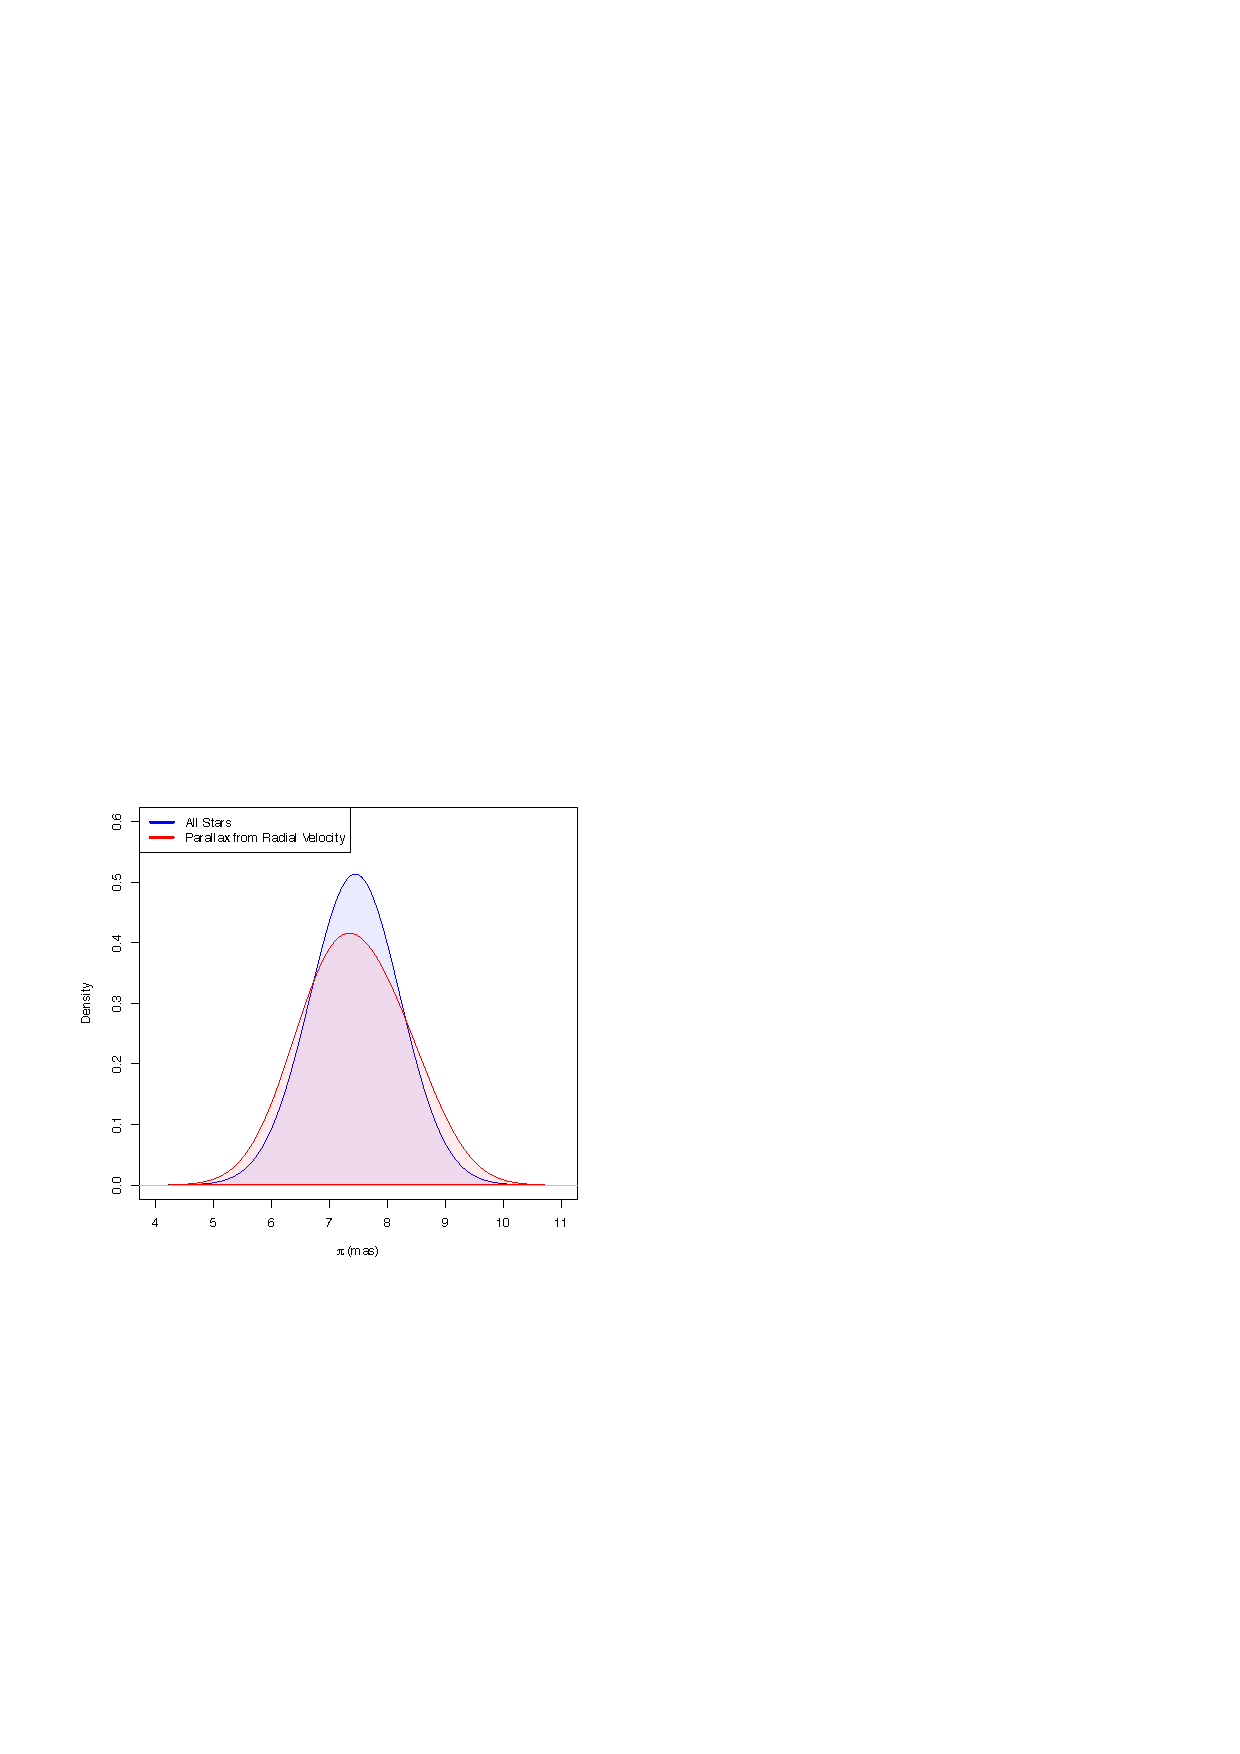
\includegraphics[height=8cm]{background/Figures/F13_Galli2017.pdf}
        \caption{Parallaxes according to \citet{Galli2017}. The red line shows all their candidate members (1210) while the blue one only those with known radial velocity (64). Reproduced from Figure 13 of \citet{Galli2017}, \textit{\usebibentry{Galli2017}{title}}, \usebibentry{Galli2017}{journal}, \usebibentry{Galli2017}{volume}.}
        \label{fig:parallaxPhillip}
    \end{subfigure}
    \begin{subfigure}[t]{\textwidth}
    \centering
       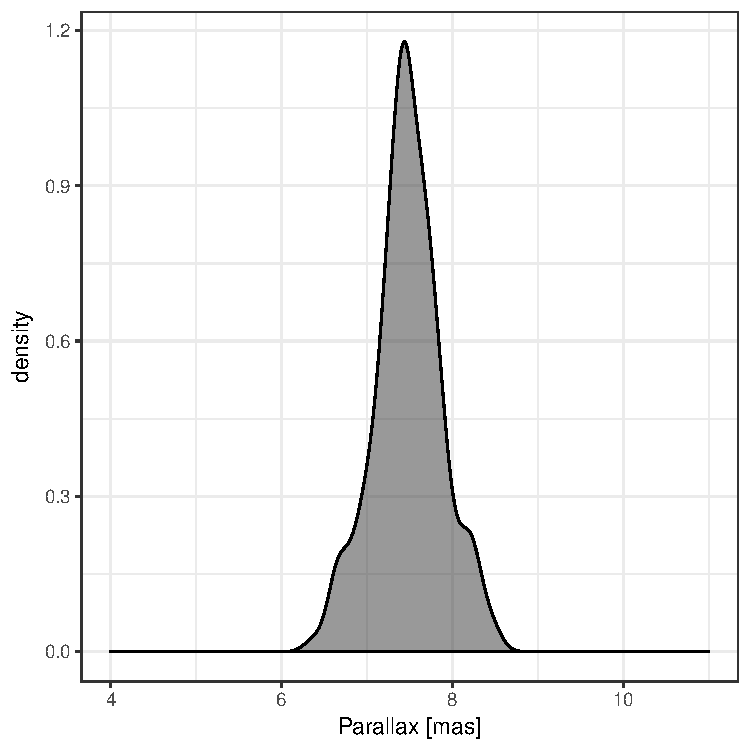
\includegraphics[height=8cm]{background/Figures/Parallax_GaiaCol2017.pdf}
        \caption{Parallaxes according to \citet{2017A&A...601A..19G}. Only their 152 candidate members.}
        \label{fig:parallaxTGAS} 
    \end{subfigure}
    \caption{Distribution of parallaxes for the Pleiades members.}
\end{figure}



\section{Spatial Distribution}
The spatial distribution is the two dimensional projection in the plane of the sky, the one perpendicular to the line of sight, of the of the cluster three dimensional space distribution. In general, individual object positions in the sphere of the sky, which are commonly known as the coordinates right ascension (R.A.) and declination (Dec.), are fare more easily measured than individual parallaxes. For this reason, just a small fraction of objects has parallaxes. For example, in the case of the Pleiades, only $\sim70$ members out of $\sim2100$ have \emph{Hipparcos}'s parallaxes. This figure comes after cross matching the candidate members of \citet{Bouy2015} with the \emph{Hipparcos} catalogue \citep{1997A&A...323L..49P}. As we saw in the previous section, this figure roughly doubled with the new \emph{Gaia} DR1 \citep{2016A&A...595A...1G}. In addition to the scarcity of parallaxes, which is expected to be solved with future \emph{Gaia} data releases, the relative uncertainties in R.A. and Dec. coordinates are far better ($10^{-5}$) than those of individual parallaxes ($10^{-1}$).

Due to the previous considerations, the space distribution of the Pleiades has been studied mainly trough its spatial distribution.
This last has been the subjects of several studies. One of the earliest results of the Pleiades spatial distribution was done by \citet{Limber1962}. He used a mixture of four indices polytropic distribution, as was described is his earlier \citet{Limber1961} work, to fit the spatial distribution of the 246 candidate members of \citet{Trumpler1921}. These candidates were contained in a $3^o$ radius around \emph{Alcyone} (one of the central most massive stars of the Pleiades cluster). 

\sloppy
Later, \citet{Pinfield1998} fitted King profiles \citep{King1962} of different masses ($5.2,1.65,0.83,0.3 \,M_{\odot}$) to candidate members from the literature which covered a $3^o$ radius area. They estimated a tidal radius of $13.1\,pc$, in which $1194$ candidate members were contained. The total mass of these members amounted to $735\,M_{\odot}$. They estimated a mean mass of $0.616\,M_{\odot}$. 

On the same year \citet{Raboud1998} also fitted a King's profile \citep{King1962} to a list of 270 candidate members contained within a $5^o$ radius area. They found a core radius of $1.5\,pc$ and a tidal radius of $17.5\,pc$. Using different approaches, they derived a total mass within the range of $500 -8000 \,M_{\odot}$. They also measured an ellipticity of $\epsilon=0.17$, however they do not made any explicit mention on the position angle of the axis of the ellipse.

Later, \citet{Adams2001} also fitted a King's profile to objects with membership probabilities $p>0.3$ within a radius of $10^o$. They found a core radius of $2.35-3.0\,pc$ and a tidal radius of $13.6-16\,pc$. They estimate a total mass of $\sim 800\,M_{\odot}$. Their measured ellipticities were in the range $0.1-0.35$. 

\citet{Converse2008} used a sample of 1245 from \citet{Stauffer2007} to fit a King's profile. They obtained a tidal radius of $18\,pc$ and a core radius of  $1.3 \,pc$. Later, \citet{Converse2010} refined their study and obtained a core radius of $2.0\pm0.1\,pc$, a tidal radius of $19.5 \pm 1.0 \,pc $ and a total mass of $870\pm35\,M_{\odot}$. In Fig. \ref{fig:spatialConverse}, I reproduce the surface density fit obtained by these authors.

The previous summary of results shows at least two interesting points. In first place, King's profile \citep{King1962} has bee the preferred choice for the Pleiades cluster, although it was created to fit the spatial distribution of globular clusters. Since globular clusters are far away than open clusters and in a low density environment, usually the end of their spatial distribution is well within the survey area. The second point concern the increasing trend of the tidal radius with the size of the survey and the publication date. As the surveys increase in area the derived tidal radii increase as well. The exception is the work of \citet{Adams2001}. Since they used low membership probability ($\geq0.3$) objects they may have also fitted the field. The surface density of a tidally truncated cluster should diminish with radius and eventually go to zero at the tidal radius. However, as can be seen in Figure \ref{fig:spatialAdams}, where I reproduce Figure 8 of \citet{Adams2001}, their surface density remains almost constant after $5^o$. This may be an indication of contamination in their sample.

The two points mentioned before are tightly related. Since so far the surveys have not reached the end of the Pleiades spatial distribution, the samples of members we currently have are spatially biased. They are not a sample of the entire cluster population but just of its central region. Thus, estimates from the King's tidal radius will be biased towards lower values until the physical end of the cluster will be within the survey's coverage. This issue will be addressed once the full sky coverage of \emph{Gaia's} data will be available.

\begin{figure}[ht!]
    \centering
    \begin{subfigure}[t]{0.49\textwidth} \centering
        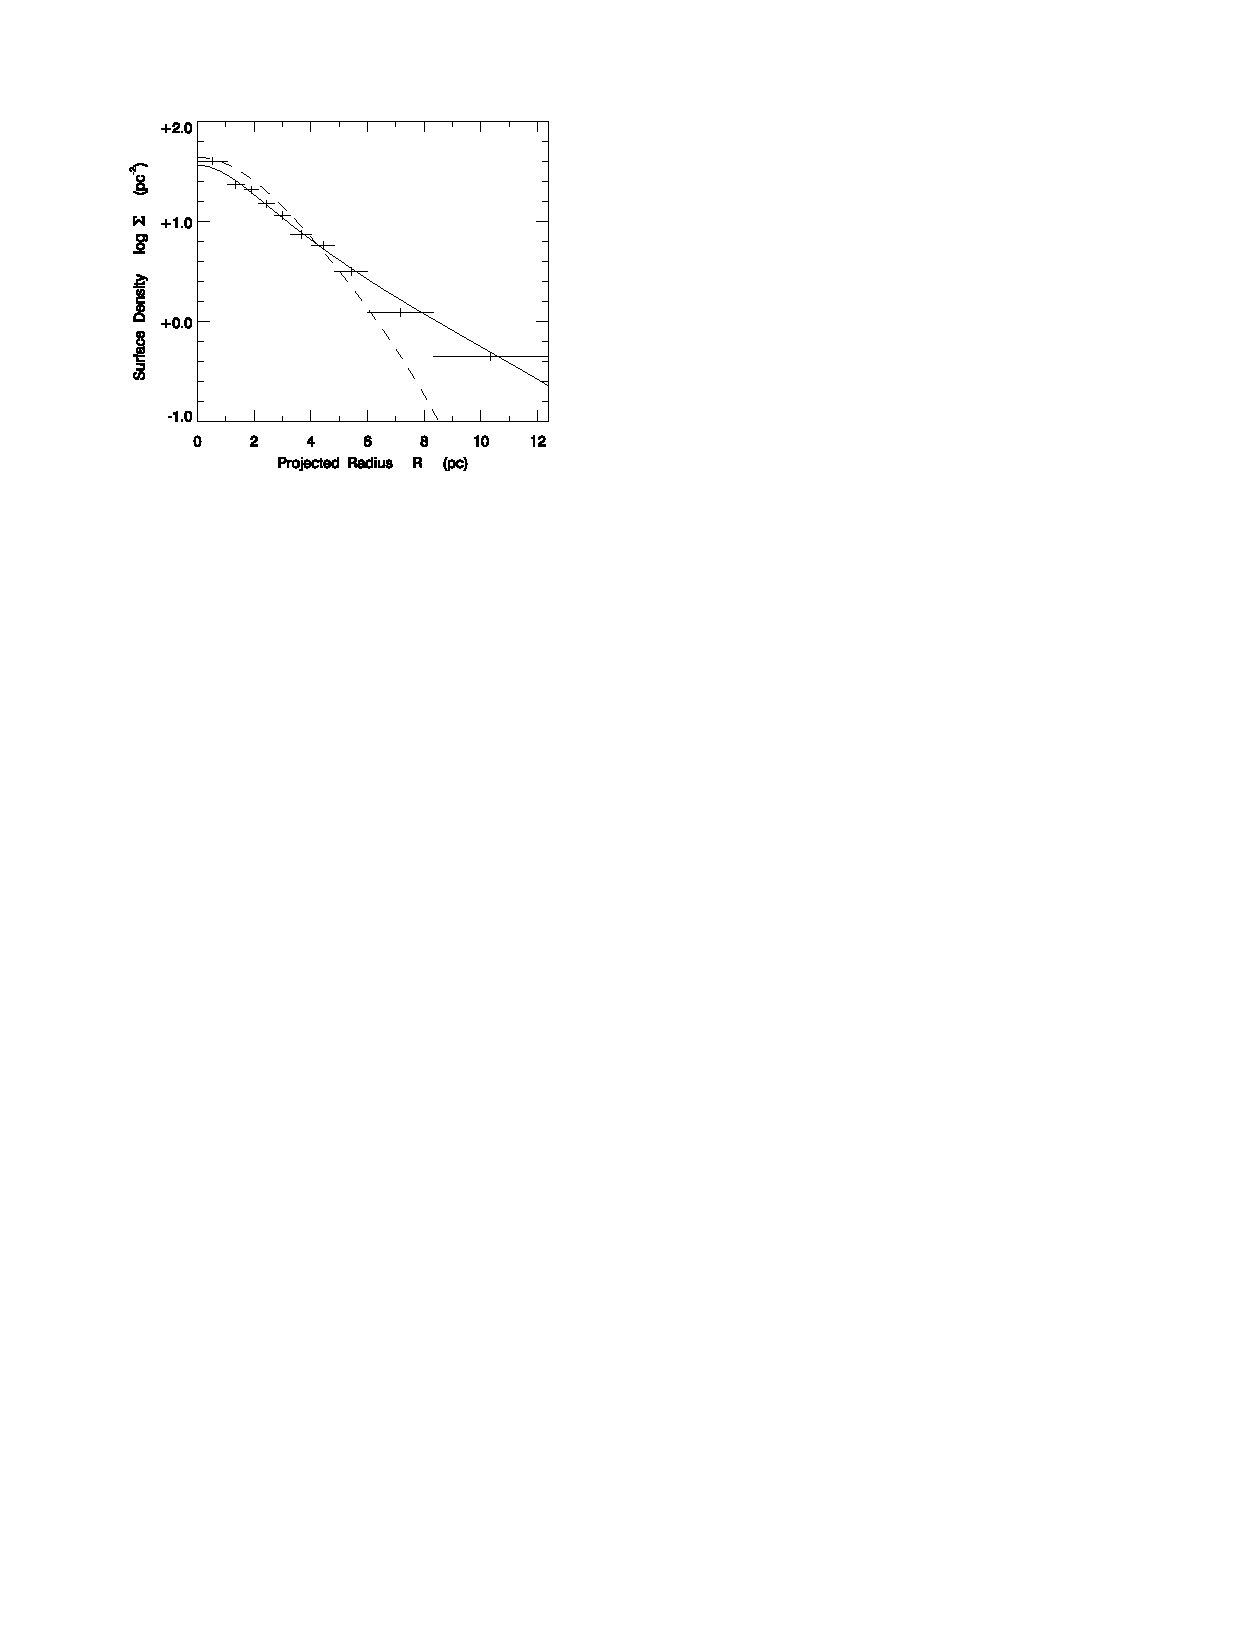
\includegraphics[height=6cm]{background/Figures/F1_Converse2010.pdf}
        \caption{Surface density according to \citet{Converse2010}. The dots and the solid line represent the data and the fitted King's profile, respectively. Reproduced from Figure 1 of \citet{Converse2010}, \textit{\usebibentry{Converse2010}{title}}, \usebibentry{Converse2010}{journal}, \usebibentry{Converse2010}{volume}.}
        \label{fig:spatialConverse}
    \end{subfigure}
    \begin{subfigure}[t]{0.49\textwidth} \centering
       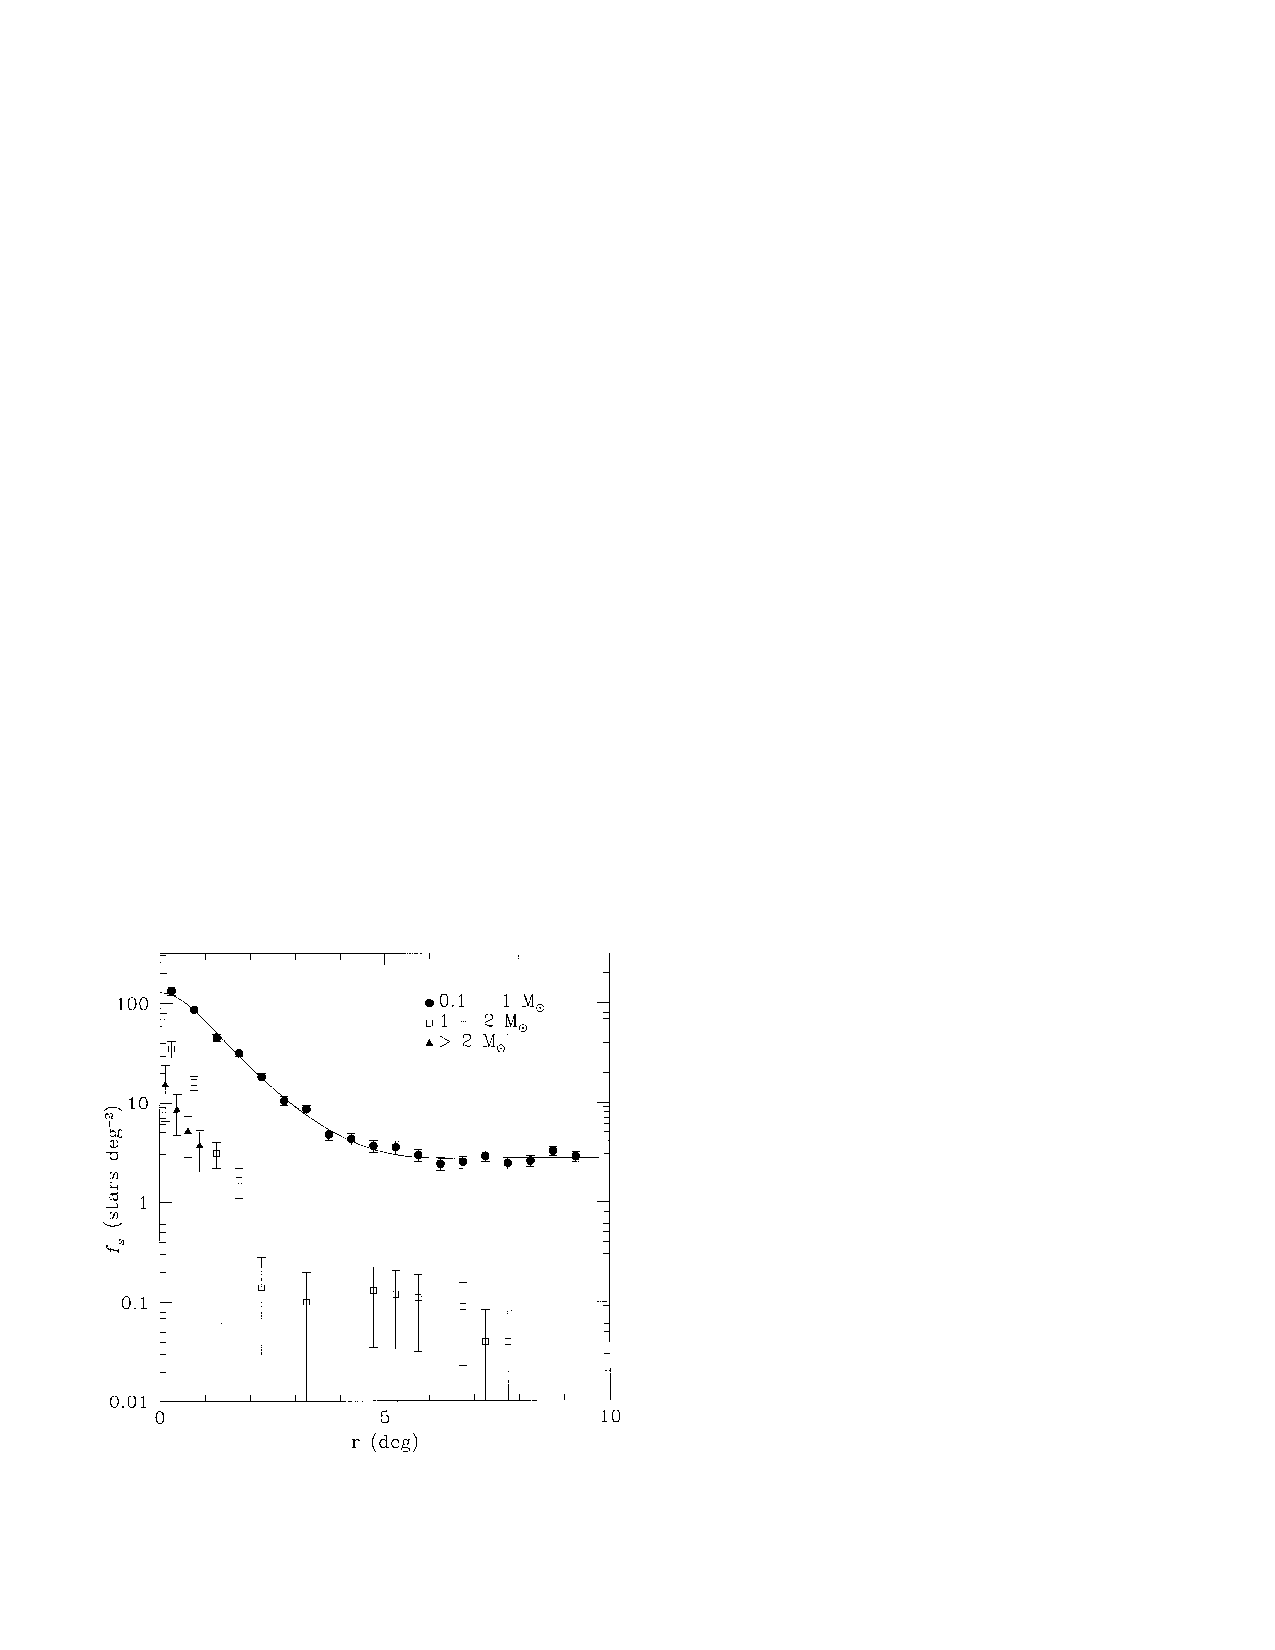
\includegraphics[height=6cm]{background/Figures/F8_Adams2001.pdf}
        \caption{Surface density according to \citet{Adams2001}. The line shows the fitted King's profile. Reproduced from Figure 8 of \citet{Adams2001}, \textit{\usebibentry{Adams2001}{title}}, \usebibentry{Adams2001}{journal}, \usebibentry{Adams2001}{volume}.}
        \label{fig:spatialAdams} 
    \end{subfigure}
    \caption{Spatial distribution of the Pleiades cluster.}
\end{figure}

  
\section{Velocity Distribution}

The three dimensional velocity distribution of the Pleiades has also been studied using its projections. One of them goes along the line of sight, which corresponds to the radial velocity, and another one, which is perpendicular to the previous one, rests in the plane of the sky. This corresponds to the proper motions. Proper motions are angular velocities obtained after measuring the angular displacement that an object shows when measured in at least in two different epochs. Again, measuring the individual stellar positions and its displacement over time is far more easy than measuring radial velocities. These are estimated by means of the Doppler shifting of the absorption lines in the spectre of the object, which means they are observationally intensive.  Despite that they are more precise than proper motion measurements (usually on the $1 \,km\cdot s^{-1}$ regime), they demand large telescopes and longer observing times. For these reasons, historically, the velocity distribution has been studied through the spatial velocity or proper motions distribution. 

Probably the first description of the spatial velocity distribution of the Pleiades is that of \citet{1884MNRAS..44..355P}. Using archival data from  Königsberg (1838-1841), Paris(1874) and Oxford (1878-1880) observatories, together with his own \emph{Differential Micrometer} observations, he was able to observe the relative displacements of 40 Pleiades stars. According to him \citep{1884MNRAS..44..355P}: \textit{the relative displacements of these distant suns, although not distinctly and accurately measurable in numerical extent, appear to vary both in direction and amount; indicating thereby the mutual influence of a group of gravitating bodies.} 

Later, \citet{Trumpler1921} use, for the first time, proper motion measurements to identify the members of the Pleiades cluster. He classified objects as candidate members according to the distance they show, in the proper motion space, to the mean proper motion of the cluster. This mean was previously calculated by Boss in his \emph{Preliminary General Catalog} \citep{Trumpler1921}. So far as my historic research went, the Boss work was the first measurement of an statistic of the spatial velocity distribution of the Pleiades. 

Later \citet{1938AJ.....47...25T}, using Trumpler's data an archival compilations, was able to measure the dispersion of the proper motions distribution. He estimated it to be $0.79\,mas\cdot yr^{-1}$. This was probably, the first measurement of the second moment of the spatial velocity distribution. From this value he then derived a total mass of $260\,M_{\odot}$.

In recent years \citet{Pinfield1998} used the velocity dispersion to probe that the cluster was in an state near to the virial equilibrium. Later, \citet{2006ARep...50..714L} used the projected radial and tangential velocity components of the spatial velocity distribution of 340 members to claim the absence of evidence for rotation, expansion or compression of the cluster. Also, he also found no evidence to support mass segregation. 

Concerning the radial velocities, the first record for the Pleiades correspond to \citet{1904ApJ....19..338A}. He measured the radial velocities of six of the most brightest stars. In modern years, the latest compilation of radial velocities from the literature is that made made by \citet{Galli2017}. This list contains measurements for 394 objects. The distribution of these radial velocities is almost gaussian with a centre at $5.6\,km \cdot s^{-1}$. 

As I will explain later in this Chapter, the complete velocity distribution is a key ingredient in the understanding of the cluster dynamics. Although, spatial and radial velocities are useful projections of the complete distribution, the dynamical analysis of the cluster demands the complete velocity distribution. In \citet{Galli2017} we provide a list of 64 cluster members with full spatial velocities. In Figure \ref{fig:velocityGalli}  I show the distribution of the three projection of these spatial velocities. 

\begin{figure}[ht!]
\begin{center}
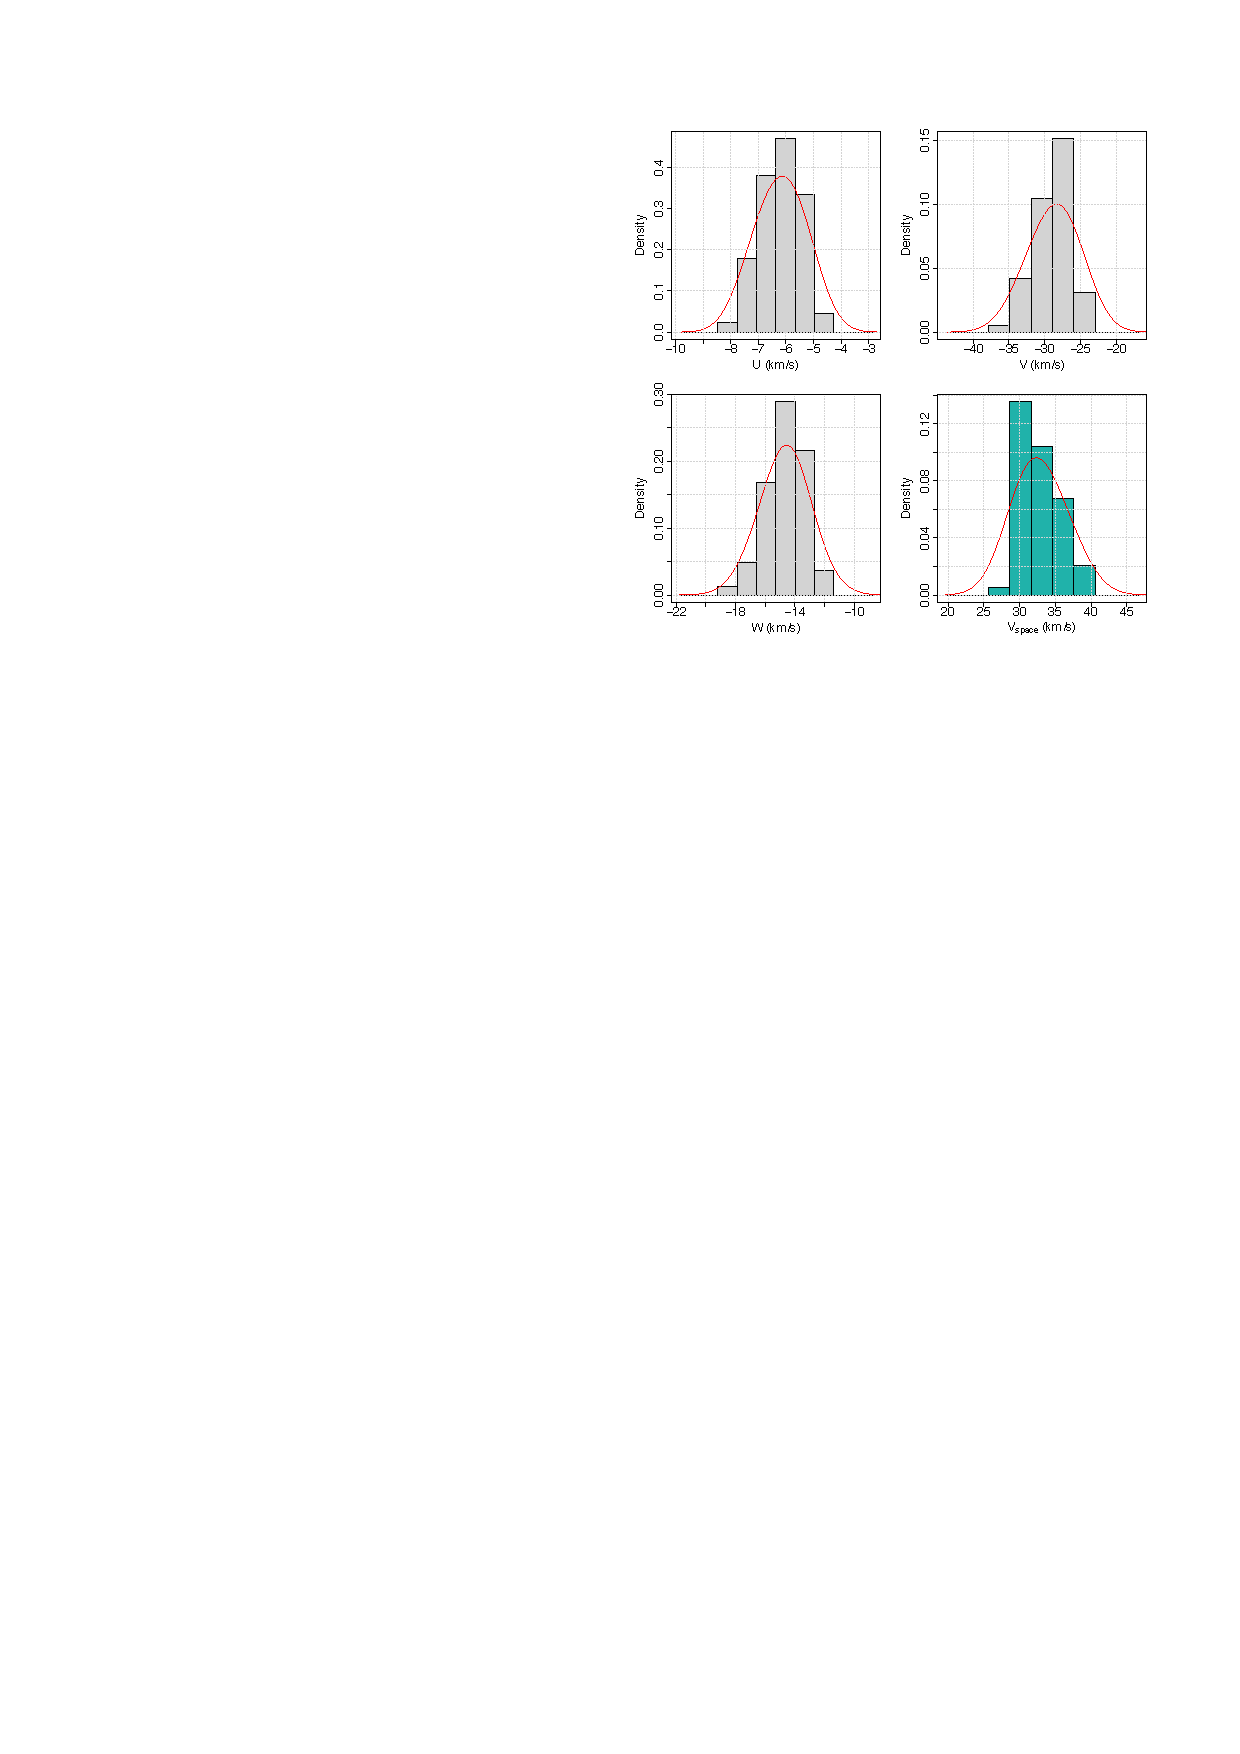
\includegraphics[width=\textwidth]{background/Figures/F11_Galli2017.pdf}
\caption{Histogram and kernel density estimation (red line) of the components (grey) and modulus (green) of the spatial velocity distribution of 64 candidate members of \citet{Galli2017} with radial velocities and parallaxes. Reproduced from Figure 11 of \citet{Galli2017},\textit{\usebibentry{Galli2017}{title}}, \usebibentry{Galli2017}{journal}, \usebibentry{Galli2017}{volume}.}
\label{fig:velocityGalli}
\end{center}
\end{figure}

\section{Luminosity Distribution}

The study of the distribution of luminosities in the Pleiades started few years later than those of the positions and proper motions. The first record I found on the luminosity distribution is the one of \citet{Trumpler1921} (see Fig. \ref{fig:luminosityTrumpler}). He computed the number of stars in each magnitude bin for his two samples of candidate members, those comprising the objects within the central $1^o$, and those within $1^o$ and $3^o$, referred as Tables I and II, respectively. The completeness of the inner sample was estimated at 14.5 magnitudes whereas that of the outer one at  9.0 magnitudes, both for the visual band. He observed that the luminosity distributions of these two samples were not alike. The inner sample is brighter than the outer one. He also observed that the luminosity distribution is not smooth and shows a local minimum at $9-10$ magnitudes, then an abrupt rise. Both effects in the two samples.

\begin{figure}[ht!]
\begin{center}
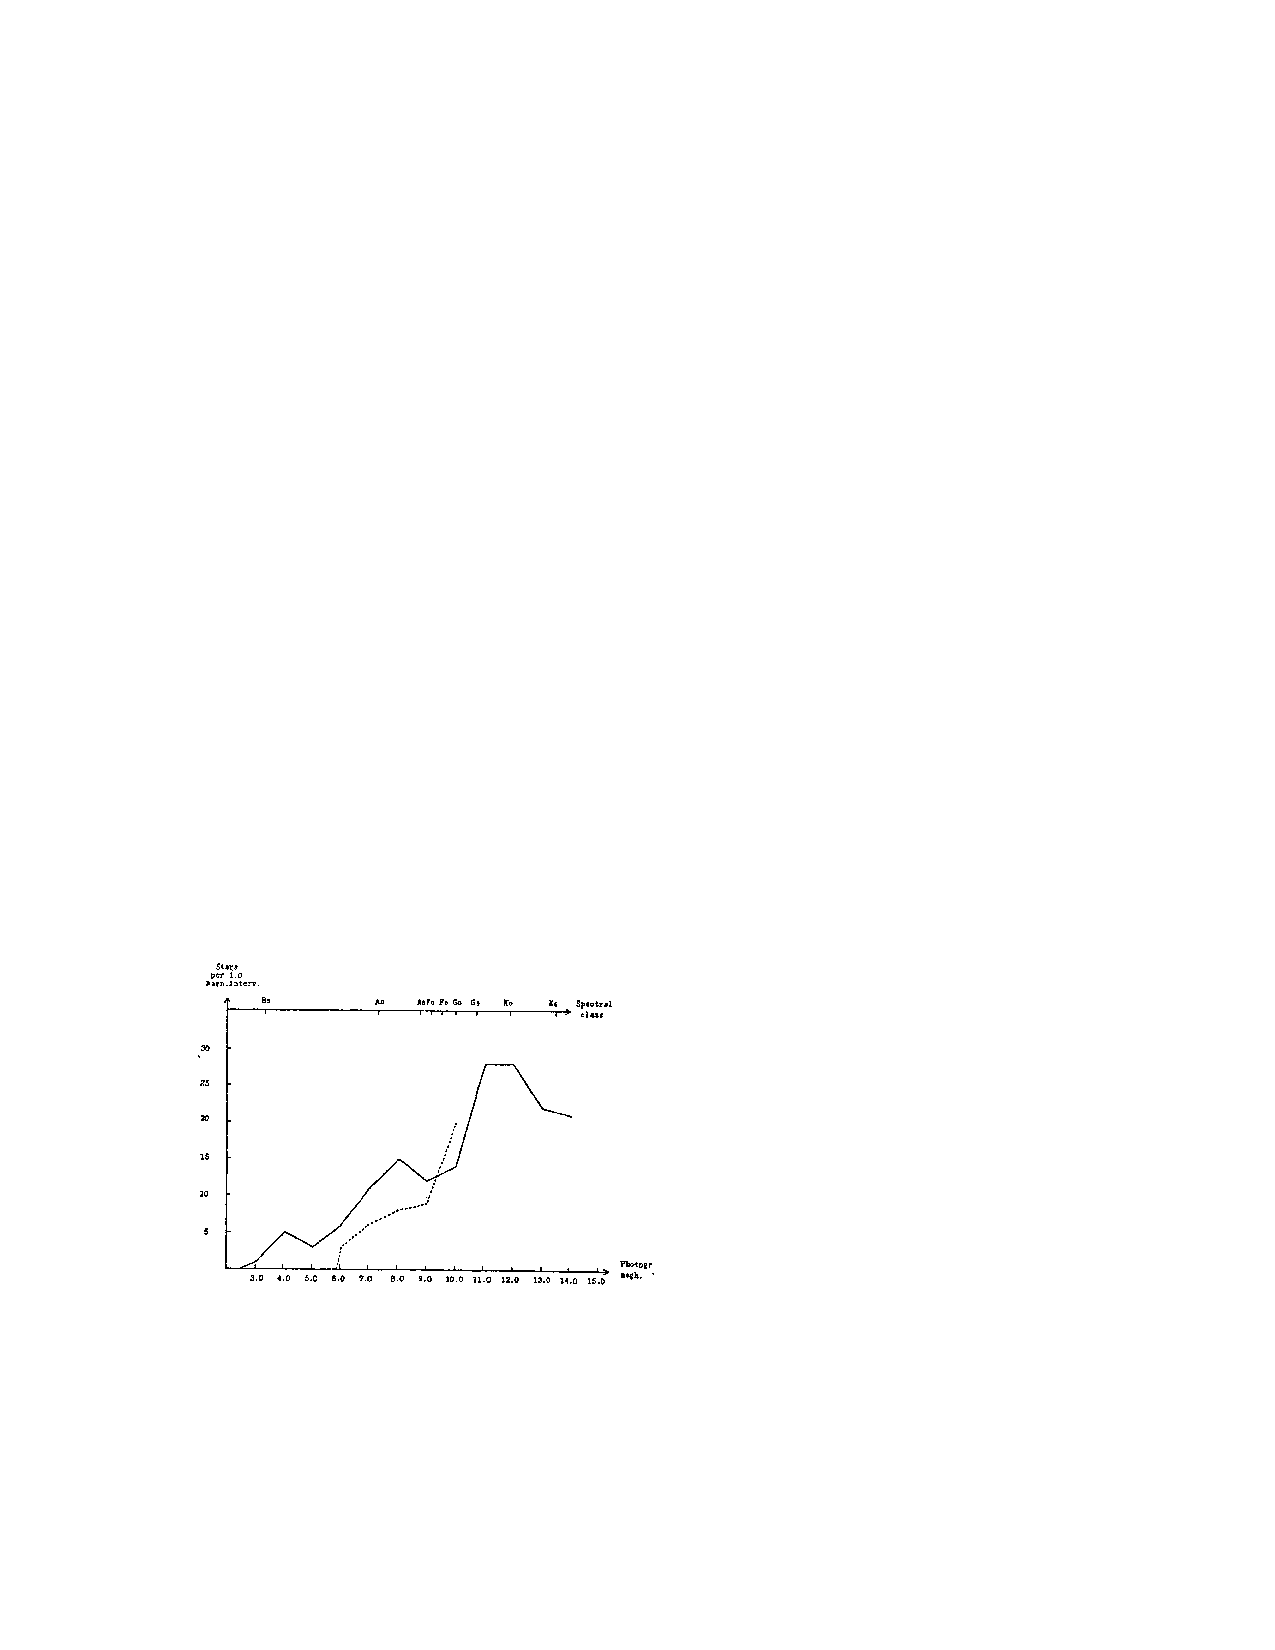
\includegraphics[width=\textwidth]{background/Figures/F2_Trumpler1921.pdf}
\caption{Luminosity distribution according to \citet{Trumpler1921}. The solid and dashed lines correspond to objects within $1^o$ and within $1^o$, and $3^o$ from the centre. Reproduced from Figure 2 of \citet{Trumpler1921},\textit{\usebibentry{Trumpler1921}{title}}, \usebibentry{Trumpler1921}{journal}, \usebibentry{Trumpler1921}{volume}.}
\label{fig:luminosityTrumpler}
\end{center}
\end{figure}

Later, \citet{Johnson1958} obtained the luminosity distribution using a sample of 289 candidate members. They assessed  membership solely on photometry. Their luminosity distribution is shown in Fig. \ref{fig:luminosityJohnson}

Later, \citet{Limber1962} compared the luminosity functions derived from the data of \citet{Trumpler1921}, \citet{Hertzsprung1947}, and \citet{Johnson1958}, with those given by the solar neighbourhood. He noted that the differences between the Pleiades and solar neighbourhood start to happen at absolute magnitude $5.5$. These distributions were complete until visual magnitudes of $8.5$ and $9.5$ mag. 

\begin{figure}[ht!]
\begin{center}
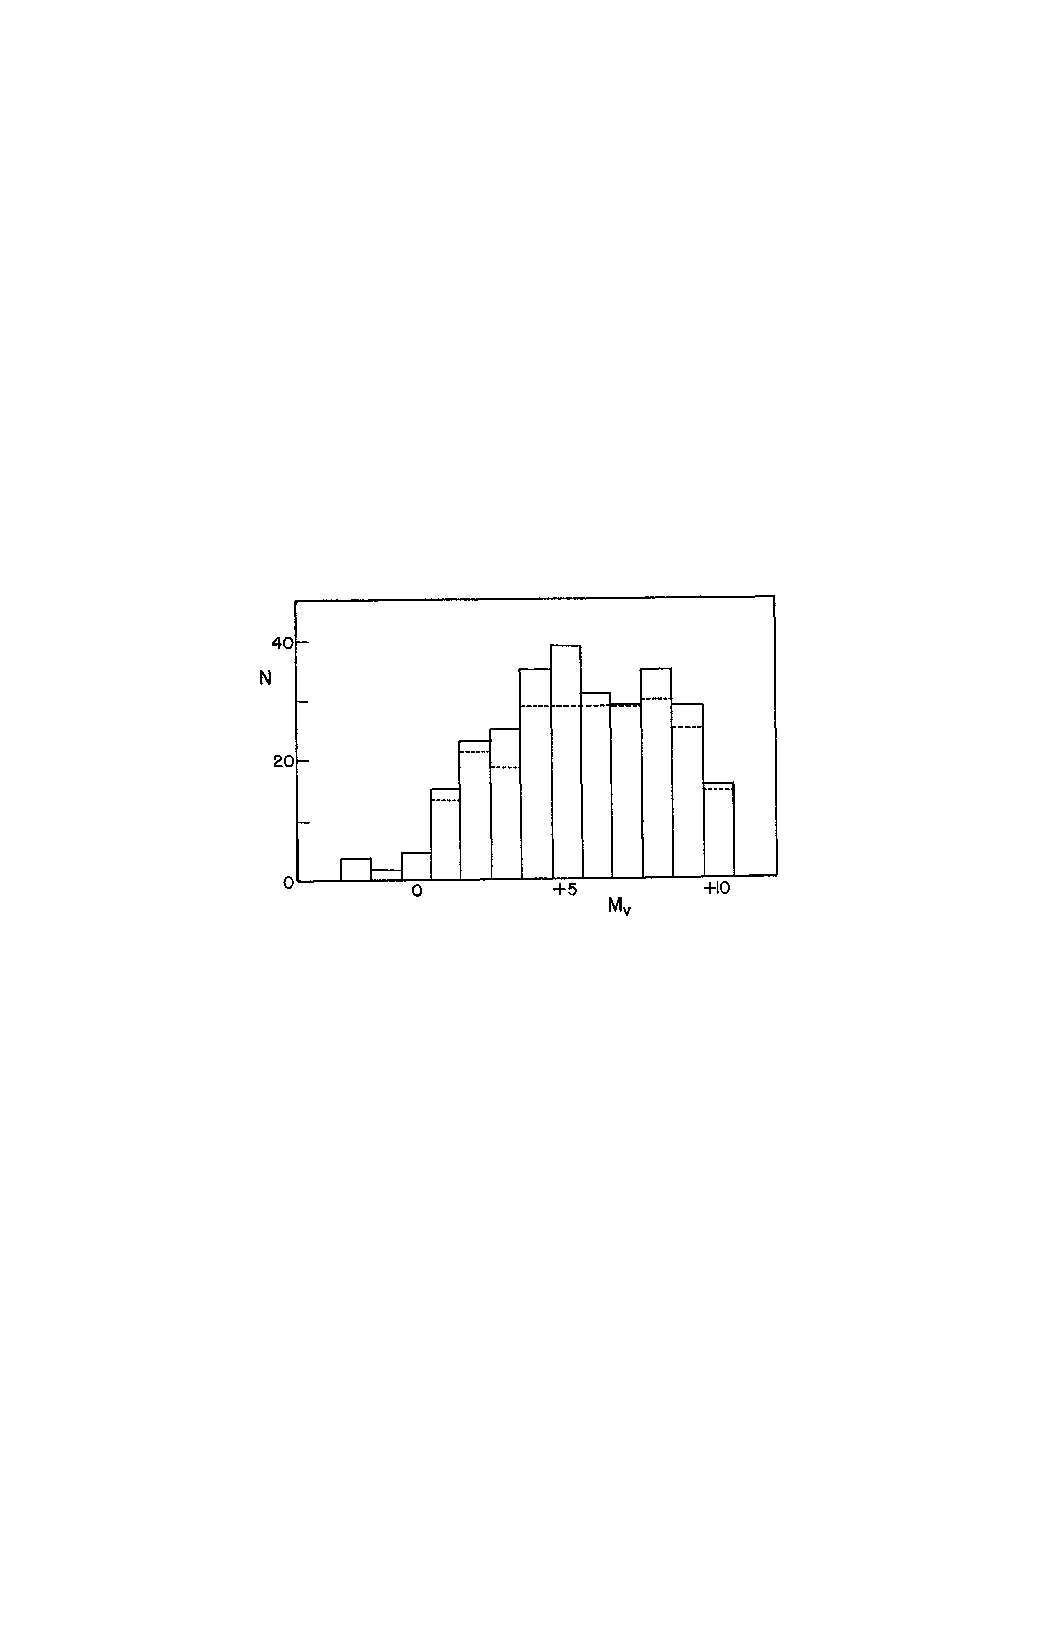
\includegraphics[height=8cm]{background/Figures/F3_Johnson1958.pdf}
\caption{Luminosity distribution in the visual band according to \citet{Johnson1958}.The dotted line represent the counts of main sequence stars only. Reproduced from Figure 3 of \citet{Johnson1958},\textit{\usebibentry{Johnson1958}{title}}, \usebibentry{Johnson1958}{journal}, \usebibentry{Johnson1958}{volume}.}
\label{fig:luminosityJohnson}
\end{center}
\end{figure}


%\begin{figure}[htbp]
%\begin{center}
%%\includegraphics[width=\textwidth]{}
%\caption{Luminosity distribution in the visual band according to \citet{Limber1962}.}
%\label{fig:luminosityLimber}
%\end{center}
%\end{figure}

In recent years, the luminosity distribution has been described in the works of \citet{Lodieu2012} and \citet{Bouy2015}. 
\citet{Lodieu2012} using the \emph{UKIDSS} DR9 survey for galactic clusters and a probabilistic members selection method (see discussion in Chapter \ref{chap:introduction}) based on proper motions, and proper motions and photometry, found 8797 and 1147 candidate members, respectively. However, they do not provide the contamination rate in their analysis. Using both lists they provide their luminosity distributions in the $Z$ band, which I show in Fig. \ref{fig:luminosityLodieu}.

\begin{figure}[ht!]
\begin{center}
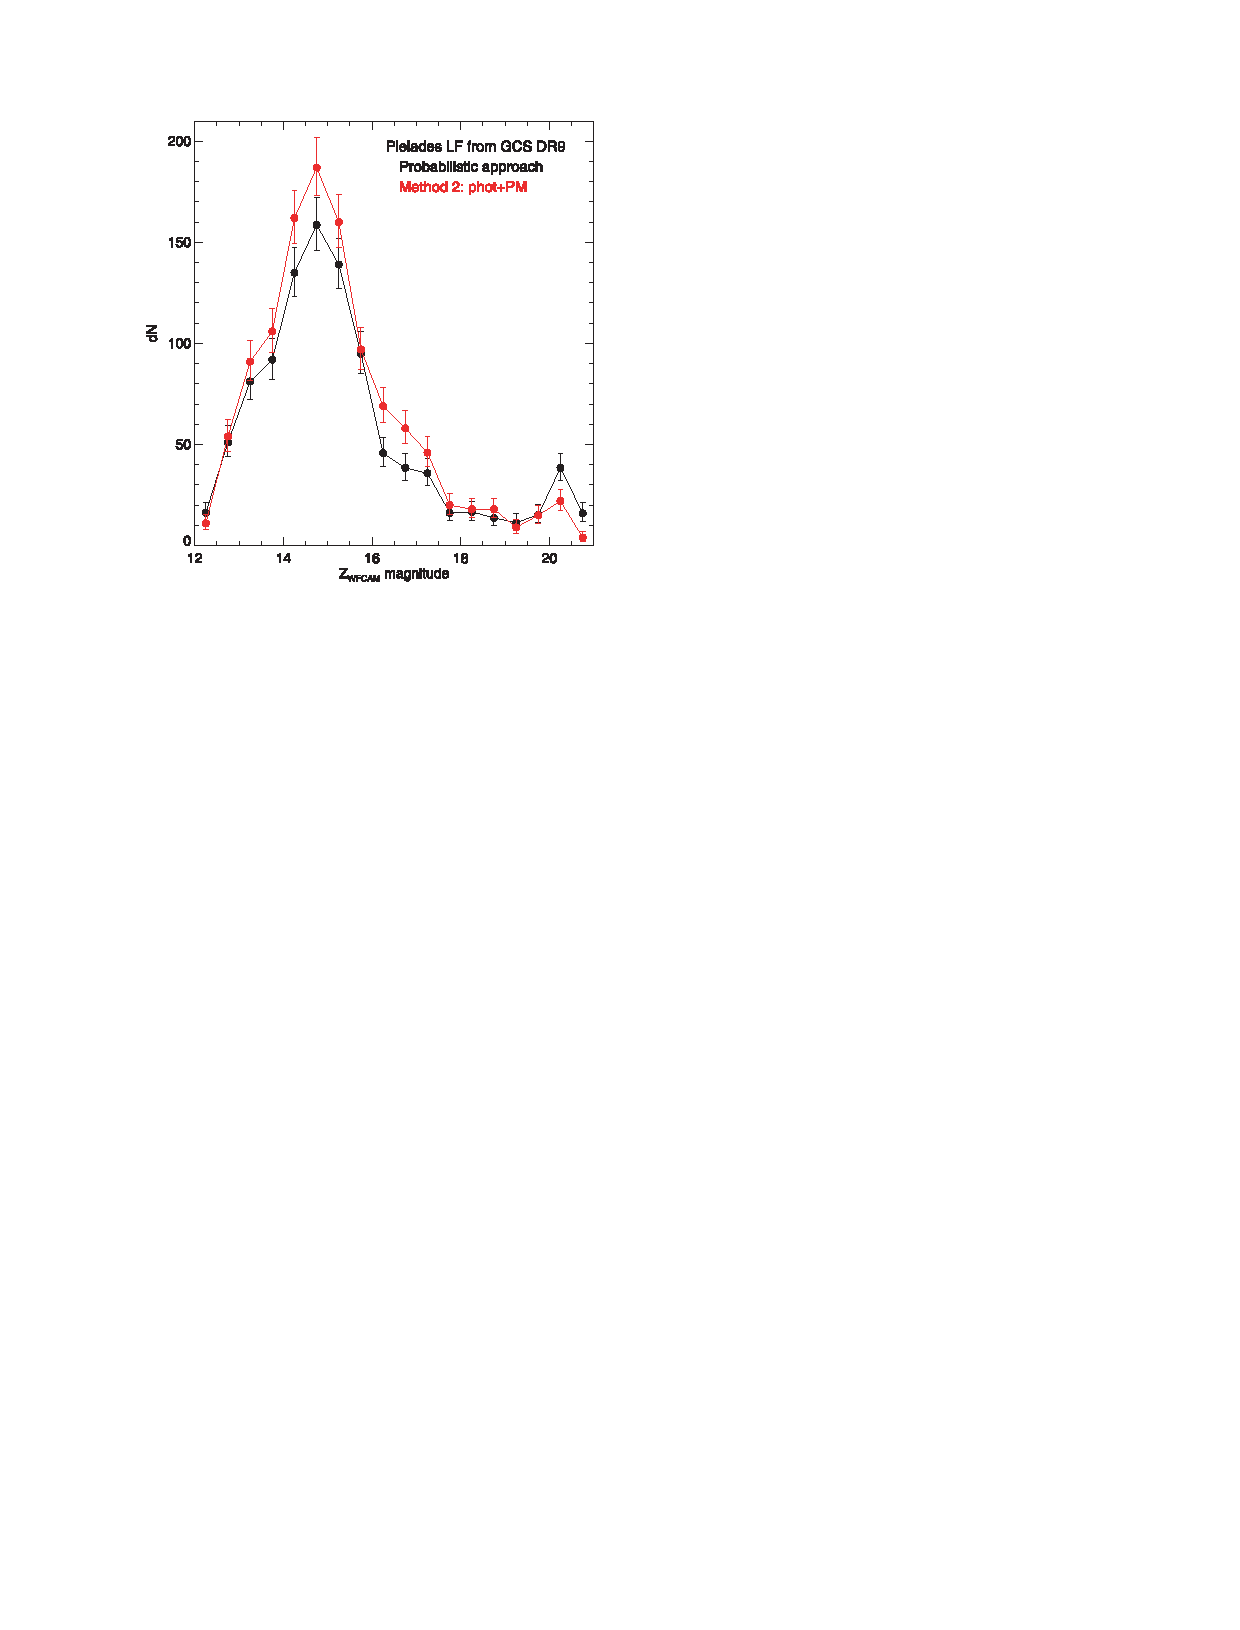
\includegraphics[height=8cm]{background/Figures/F9_Lodieu2012.pdf}
\caption{Luminosity distribution  in the $Z$ band according to \citet{Lodieu2012}. The red and black lines correspond to the two different probabilistic methods.  Reproduced from Figure 9 of \citet{Lodieu2012},\textit{\usebibentry{Lodieu2012}{title}}, \usebibentry{Lodieu2012}{journal}, \usebibentry{Lodieu2012}{volume}.}
\label{fig:luminosityLodieu}
\end{center}
\end{figure}

In \citet{Bouy2015},  we estimated the present day system luminosity distribution of 1378 candidate members contained within the central $3^o$ region (with the centre at $RA=03:46:48$ and $Dec=24:10:17$ J2000.0). It is called systemic because it has not been corrected for unresolved systems. An unresolved system is a group of stars (e.g. binaries) that due to its compactness appears as a single object. This distribution was computed for the $K_s$ band and is sensitive up to $K_s \sim 20 \ \ mag$ and complete until $K_s \sim 17\ \ mag$. This luminosity distribution is reproduced in Fig. \ref{fig:luminosityBouy}


\begin{figure}[ht!]
\begin{center}
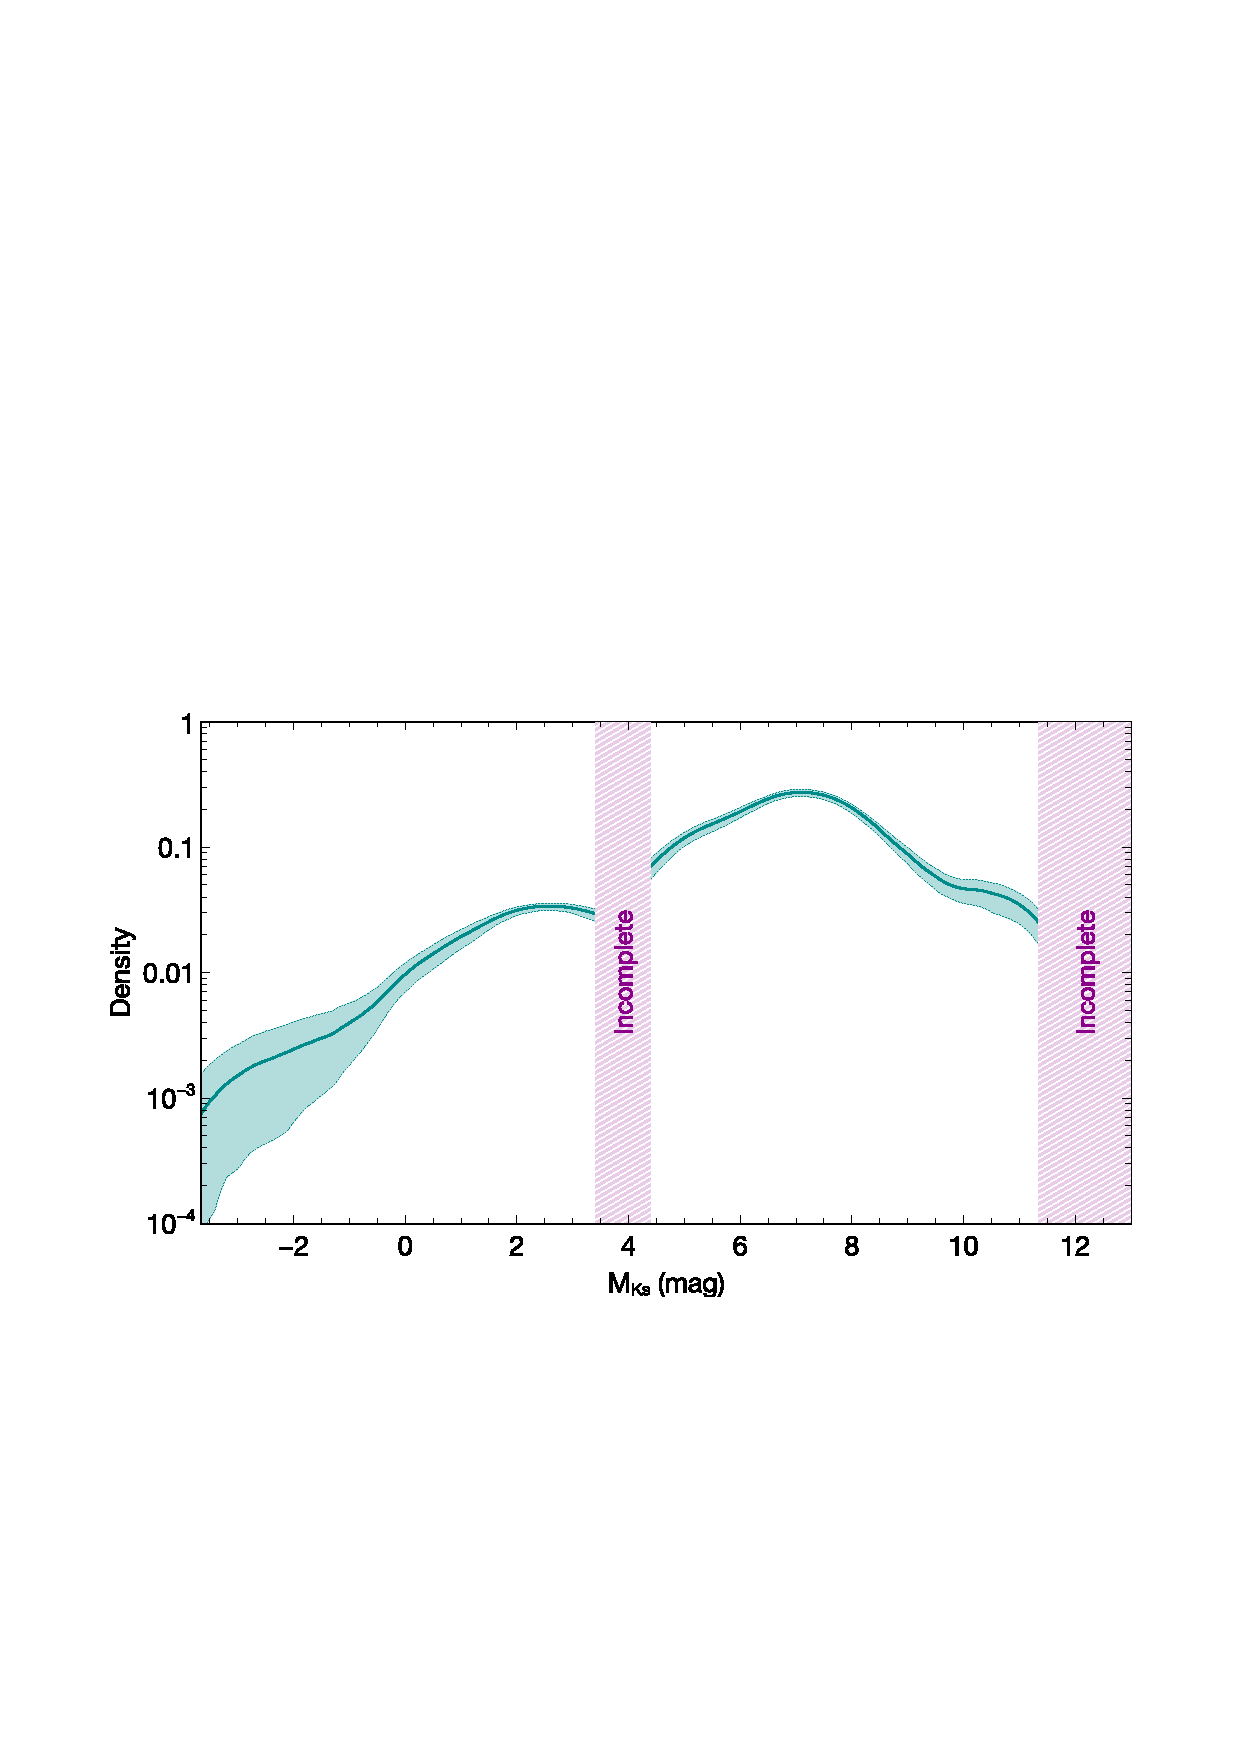
\includegraphics[width=\textwidth]{background/Figures/F8_Bouy2015.pdf}
\caption{Luminosity distribution in the $K_s$ band according to \citet{Bouy2015}. The incompleteness regions are shaded. Reproduced from Figure 8 of \citet{Bouy2015},\textit{\usebibentry{Bouy2015}{title}}, \usebibentry{Bouy2015}{journal}, \usebibentry{Bouy2015}{volume}.}
\label{fig:luminosityBouy}
\end{center}
\end{figure}

\section{Mass Distribution}

In astrophysics, the mass distribution is a cornerstone in the understanding of the star formation process and the later evolution of stellar systems. Although the temporal evolution of these systems is mainly dominated by the gravitational potential, the initial conditions and an ongoing star formation process, if any, can contribute to the shape of the mass distribution. This last contains the fingerprints of past events in the history of the cluster and plays a key roll in its future evolution. Indeed, the mass distribution is essential in one of modern astrophysics' objectives: the determination of the roll played by the initial conditions or the environment, in the temporal evolution of the stellar systems. Furthermore, the initial mass distribution is a key element in the study of galactic and extragalactic populations.  

The mass distribution of the Pleiades has been largely studied. The first work on the mass distribution is that of \citet{Limber1962}. Although he did not shows any graphical or tabular representation of it, he gave the luminosity distribution and the mass-luminosity ratio. Form these the mass distributions can be derived. Instead, he use them to obtain the total mass of the cluster ($760\,M_{\odot}$,see next Section). 

Most probably, the first work to present the mass distribution derived from luminosity distributions and a mass-luminosity relation from theoretical models was that of \citet{Hambly1991}. Using $R$ and $I$ observations from the \emph{United Kingdom Schmidt Telescope Unit} together with the mass-luminosity relation from theoretical isochrone models of Padova group, he was able to transform his luminosity distribution into a mass distribution. In Fig. \ref{fig:massHambly}, I reproduce his results. 

\begin{figure}[ht!]
\begin{center}
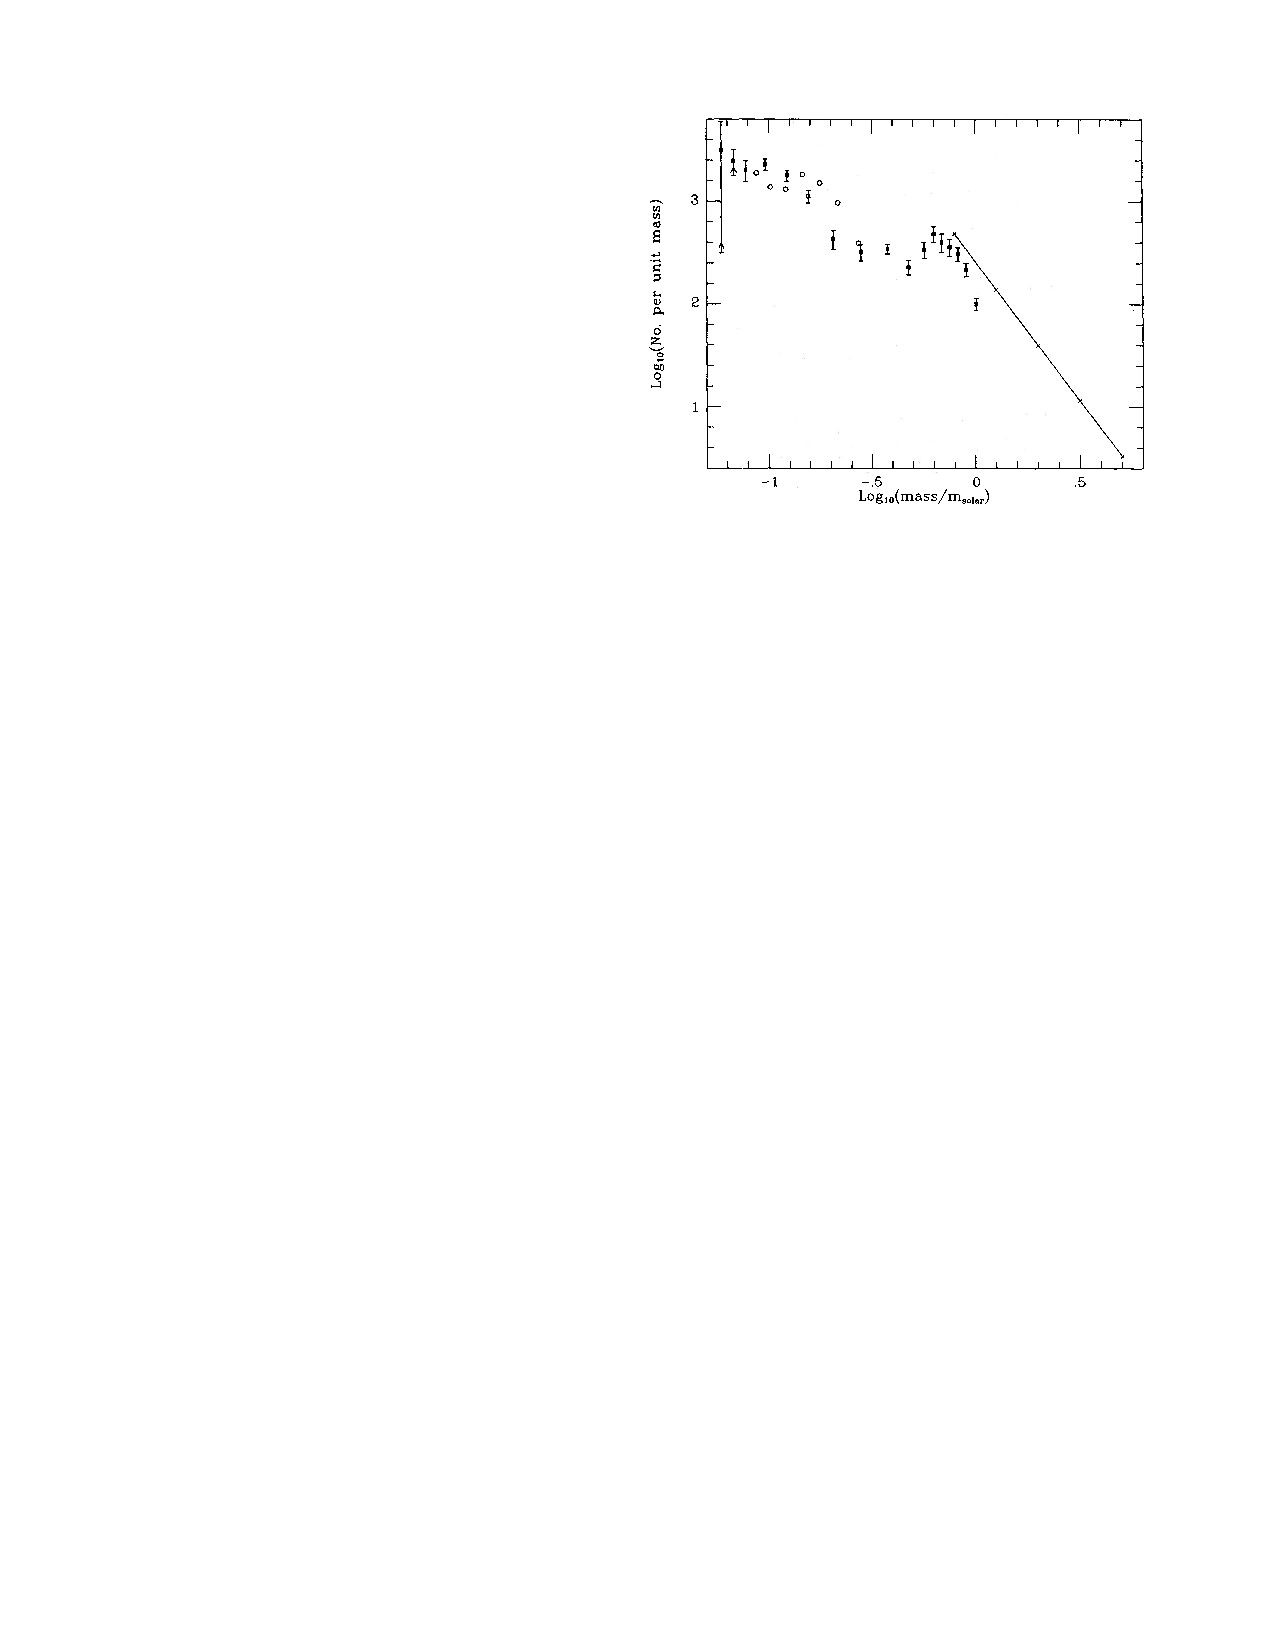
\includegraphics[height=8cm]{background/Figures/F11_Hambly1991.pdf}
\caption{Mass distribution of \citet{Hambly1991} derived from luminosity distribution and theoretical isochrone models. The open circles result from assuming an older age of $200\,Myr$. The line represent the mass distribution of \citet{1980IAUS...85..157V}. Reproduced from Figure 11 of \citet{Hambly1991},\textit{\usebibentry{Hambly1991}{title}}, \usebibentry{Hambly1991}{journal}, \usebibentry{Hambly1991}{volume}.}
\label{fig:massHambly}
\end{center}
\end{figure}

From the year 2000 till date several studies have been published in which the subject of analysis is the Pleiades mass distribution, e.g. \citet{2000ASPC..198...59H, 2002MNRAS.335..853J, 2003A&A...400..891M, 2004A&A...426...75M, 2007MNRAS.380..712L}. However, for the sake of simplicity, here I only analyse the two most recent works, those of \citet{Lodieu2012} and \citet{Bouy2015}. The mass distributions derived from both these works are shown in Figs. \ref{fig:massLodieu} and \ref{fig:massBouy}. Both works obtained first the luminosity distribution, and then transformed it into a mass distributions using theoretical isochrone models. 

\citet{Lodieu2012} used a distance of $120.2\,pc$, an age of $120\, Myr$, and the \emph{NEXTGEN} theoretical models of \citet{1998A&A...337..403B} to transform the luminosity into the mass distribution. On the other hand, in \citet{Bouy2015} we use a distance of $136.2\,pc$ an age of $120\,Myr$ and the \emph{BT-Settl} theoretical isochrone models of \citet{2014IAUS..299..271A}. 


Both works found contrasting aspects in their discussions. In one hand \citet{Lodieu2012} found that their present day mass distribution agrees with previous studies from the literature, and is also consistent with the system field mass function of \citet{Chabrier2005}. \citet{Chabrier2005} found his function by fitting a log-normal function to the visual luminosity distribution of the closest $8 \,pc$ field objects. On the other hand, in \citet{Bouy2015} we found that although the \citet{Chabrier2005} mass function match that of the Pleiades in the $0.02-0.6\,M_{\odot}$ mass range, it predicts to many low-mass stars and brown dwarfs. 

The difference between both Pleiades present day mass distributions could arise from the different samples of members,  the different theoretical isochrone models, or from both of them. The distance values used in these works can not account for the observed differences since they introduce only a general shift in the luminosity. 

Concerning the differences between the two isochrone models, in \citet{2013MmSAI..84.1053A} the authors show there are clear differences between the effective temperatures delivered by the \emph{BT-Settl} and the \emph{NEXTGEN} model in the low-mass regime at $5 \,Gyr$.  

Concerning the differences between the lists of candidate members, in one hand \citet{Lodieu2012} do not provide (at least explicitly) any estimate of contamination rate of their samples. Furthermore, their membership methodology has some draw-backs \cite[see][]{Sarro2014} that may have biased their results. Therefore, the agreement that \citet{Lodieu2012} found between their present day mass distribution and the one of \citet{Chabrier2005}, which models the field mass distribution, seem to indicate at least the following options. The Pleiades present day mass distribution indeed follows the field mass distribution. Or, the sample of candidate members of \citet{Lodieu2012} is contaminated by the field, thus resembles it.  

On the other hand, in \citet{Bouy2015} we estimated a contamination rate of 7\%. However, we have no evidence for it to be non-homogeneous. Even if the 7\% contaminants were not homogeneous distributed in the mass range, its value is not able to account for the observed discrepancies ($30-40\%$ in the low-mass regime) between the \citet{Chabrier2005} mass function and our present day mass distribution.

The previous studies show that there is still work to do in the analysis of the Pleiades mass distribution, particularly at the low-mass range where the theoretical models, both of mass function and isochrones, led to discrepancies in the present day mass distribution.  

\begin{figure}[ht!]
\begin{center}
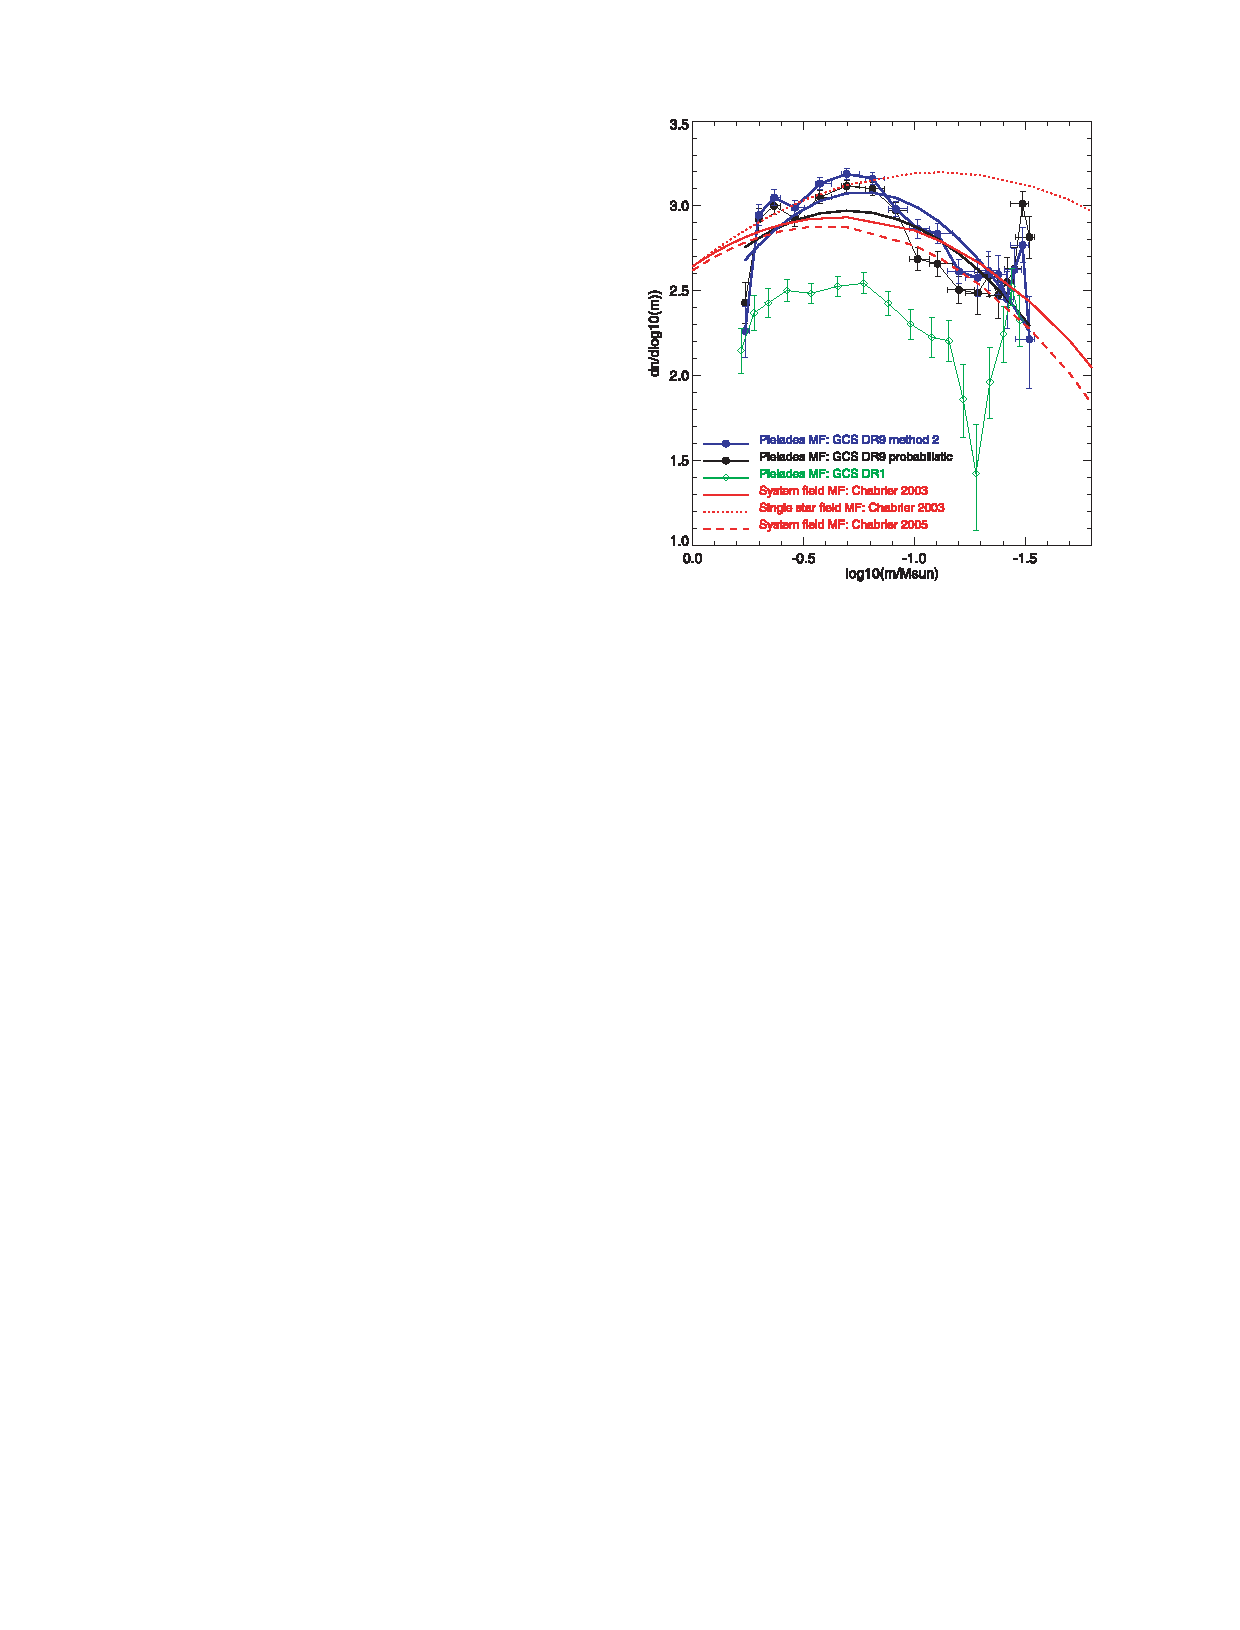
\includegraphics[height=8cm]{background/Figures/F9b_Lodieu2012.pdf}
\caption{Pleiades present day mass distribution from \citet{Lodieu2012}. GCS stands for Galactic Cluster Survey. Reproduced from Figure 9 of \citet{Lodieu2012},\textit{\usebibentry{Lodieu2012}{title}}, \usebibentry{Lodieu2012}{journal}, \usebibentry{Lodieu2012}{volume}.}
\label{fig:massLodieu}
\end{center}
\end{figure}

\begin{figure}[ht!]
\begin{center}
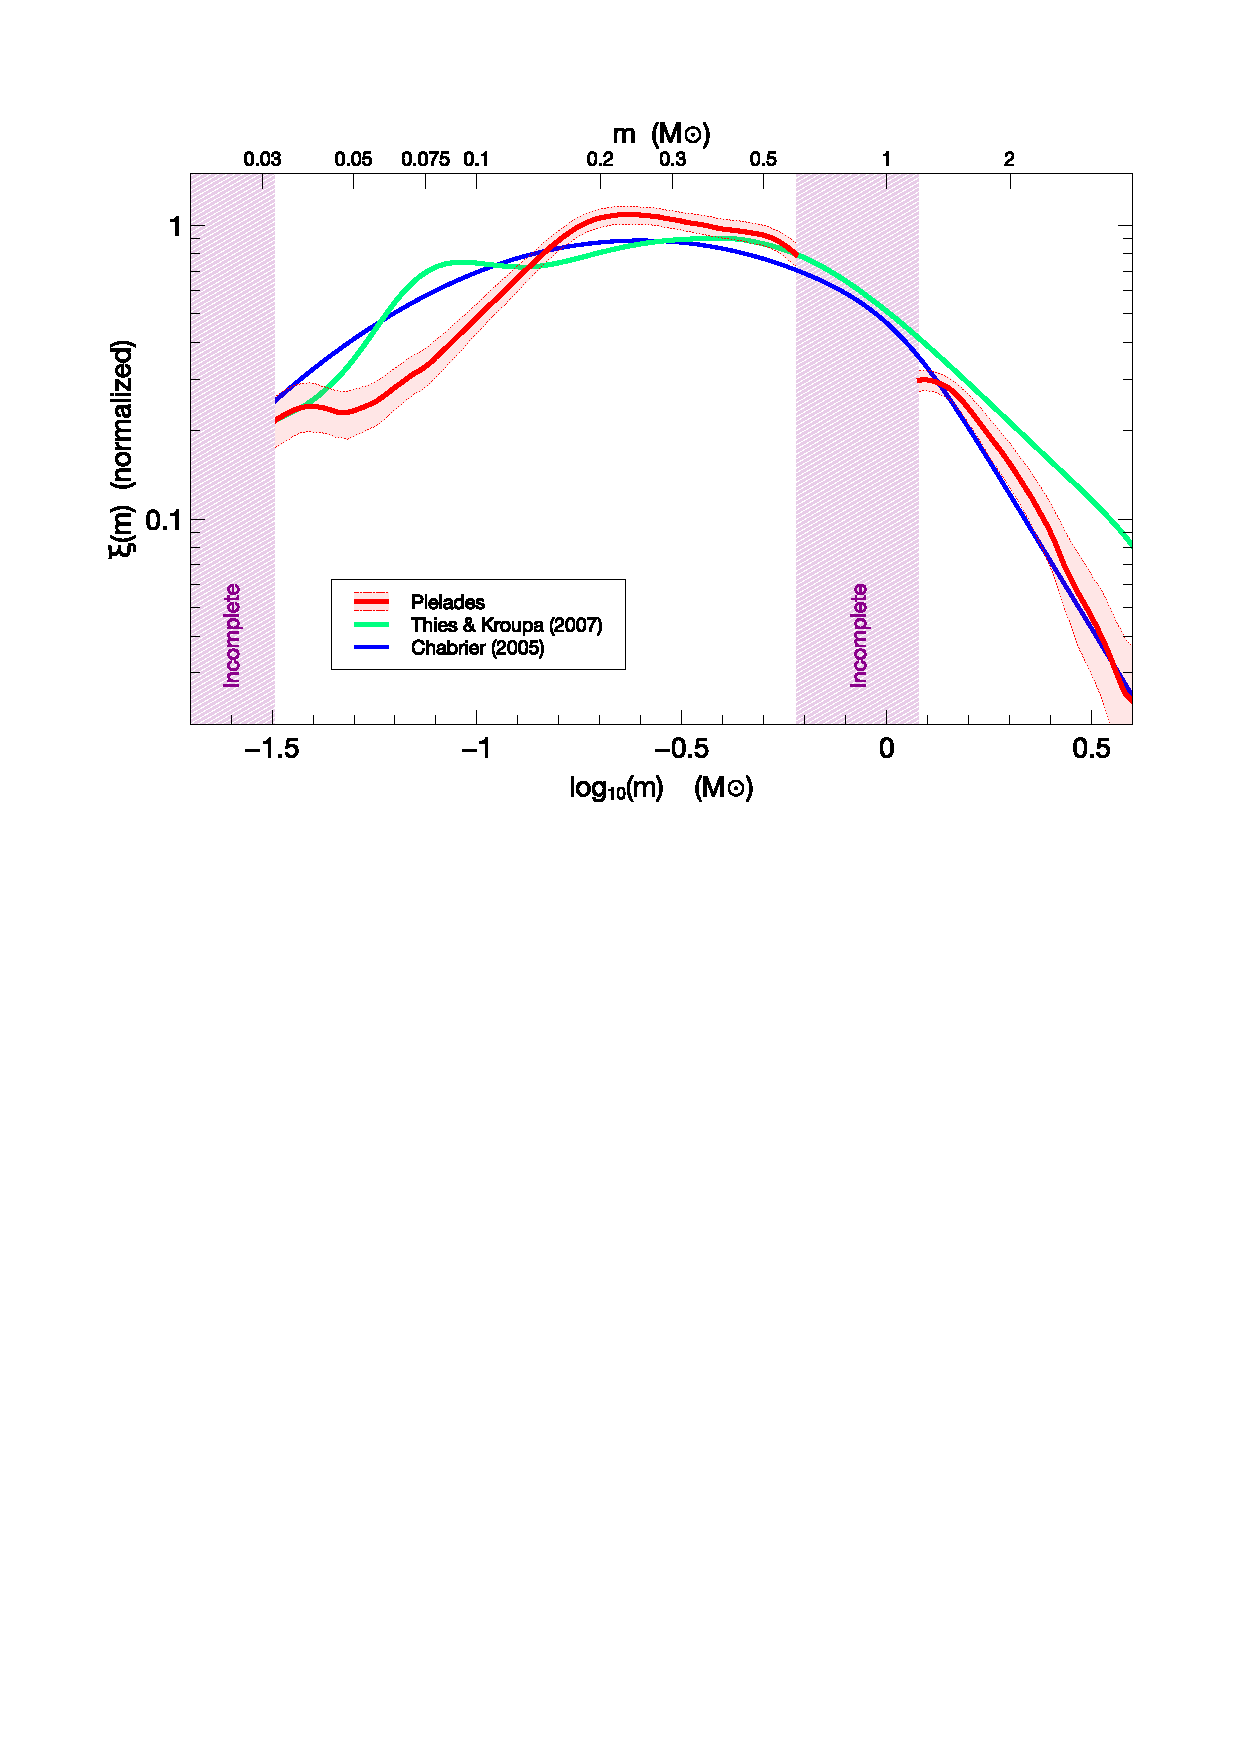
\includegraphics[height=8cm]{background/Figures/F9_Bouy2015.pdf}
\caption{Pleiades present day mass distribution  from \citet{Bouy2015} (red). IMFs from \citet{Chabrier2005}(blue) and \citet{Thies2007} (green) are also shown. Reproduced from Figure 9 of \citet{Bouy2015},\textit{\usebibentry{Bouy2015}{title}}, \usebibentry{Bouy2015}{journal}, \usebibentry{Bouy2015}{volume}.}
\label{fig:massBouy}
\end{center}
\end{figure}

\subsection{Total mass of the cluster}
Before ending this section I present a (non exhaustive) summary of the studies that provided an estimate of the total mass of the cluster.

The first record I found of the cluster total mass is that of \citet{1938AJ.....47...25T}. He estimated a total mass of $260 \,M_{\odot}$ assuming virial equilibrium. He also computed $200 \,M_{\odot}$ using the Eddignton's mass-luminosity relation for objects brighter than $15 \,mag$ in the visual band.

The subsequent works continue to report higher masses. \citet{1956MNRAS.116..296W} estimated a total mass of $337 \,M_{\odot}$ using a polytrope model fitted to Hertzsprung's catalogue. He then mentions that taking into account Trumpler's data, the total mass should be about $500\,M_{\odot}$. 

\citet{Limber1962} computed the total mass in two ways. In the first one he assumed the cluster was virialised and obtained a mass of $900 \,M_{\odot}$. Using the luminosity function he estimated the lower limit to the total mass in $760 \,M_{\odot}$. 

\citet{1970AJ.....75..563J} measured $470\,M_{\odot}$ and $690\,M_{\odot}$ using the luminosity distribution and the virial theorem, respectively. 

\citet{1980IAUS...85..157V}  determined a total mass of $2000 \,M_{\odot}$ using the virial theorem, a mean individual mass of $2\,M_{\odot}$, and a velocity dispersion of $0.7\,km \cdot s^{-1}$ in each spatial direction. 

\citet{1995JKAS...28...45L} measured $700 \,M_{\odot}$ using the luminosity distribution and a mass-luminosity relation. 

\citet{Pinfield1998} fitting a King's profile to the spatial distribution of the cluster members obtained $735\,M_{\odot}$. 

\citet{Adams2001} counting individual masses of candidate members within $5.5^o$ obtained a total mass of $690 \,M_{\odot}$. 

\citet{Converse2008} found $820 \,M_{\odot}$ after adding the individual masses of 1245  candidate members of \citet{Stauffer2007}. To obtain these masses they  transformed the $K$ and $I-K$ magnitude and colour into masses using the mass-luminosity relation given by the theoretical isochrone models of \citet{1998A&A...337..403B}. Later, \citet{Converse2010} they redo their analysis and found the total mass to be $870\pm35\ \ M_{\odot}$.

%\section{The current dynamical scenario}
%The most important sources of gravitational interactions affecting individual objects are due to: other individual objects (like for example close encounters or binary interactions), the ensemble of individual objects (the potential of the cluster itself or its momentum), other ensembles of objects (interactions with other clusters or molecular clouds) and, the galactic potential (perturbations due to the disk, resonances, arms).
%
%\subsection{Pleiades time-scales}
%Pinfield equation 13 and 14

\section{The Pleiades DANCe DR2}
\label{sect:DR2}

The Pleiades DANCe DR2 contains astrometric (stellar positions and proper motions) and photometric ($ugrizYJHK_s$) measurements for 1,972,245 objects. As explained in Chapter 1, the DANCe data set has an heterogenous origin as can be seen from Fig. \ref{fig:originDANCeDR2}. The interested reader can find more the details of this data set and its processing on \citet{Bouy2013}. Here I briefly summarise its properties. Table \ref{tab:DR2properties} contains the basic statistics for the observables, while Table \ref{tab:DR2uncertainties} does it for the uncertainties. As an example, Fig. \ref{fig:pmuncert} shows the proper motions uncertainties as a function of the $i$ magnitude.

\begin{figure}[ht!]
\begin{center}
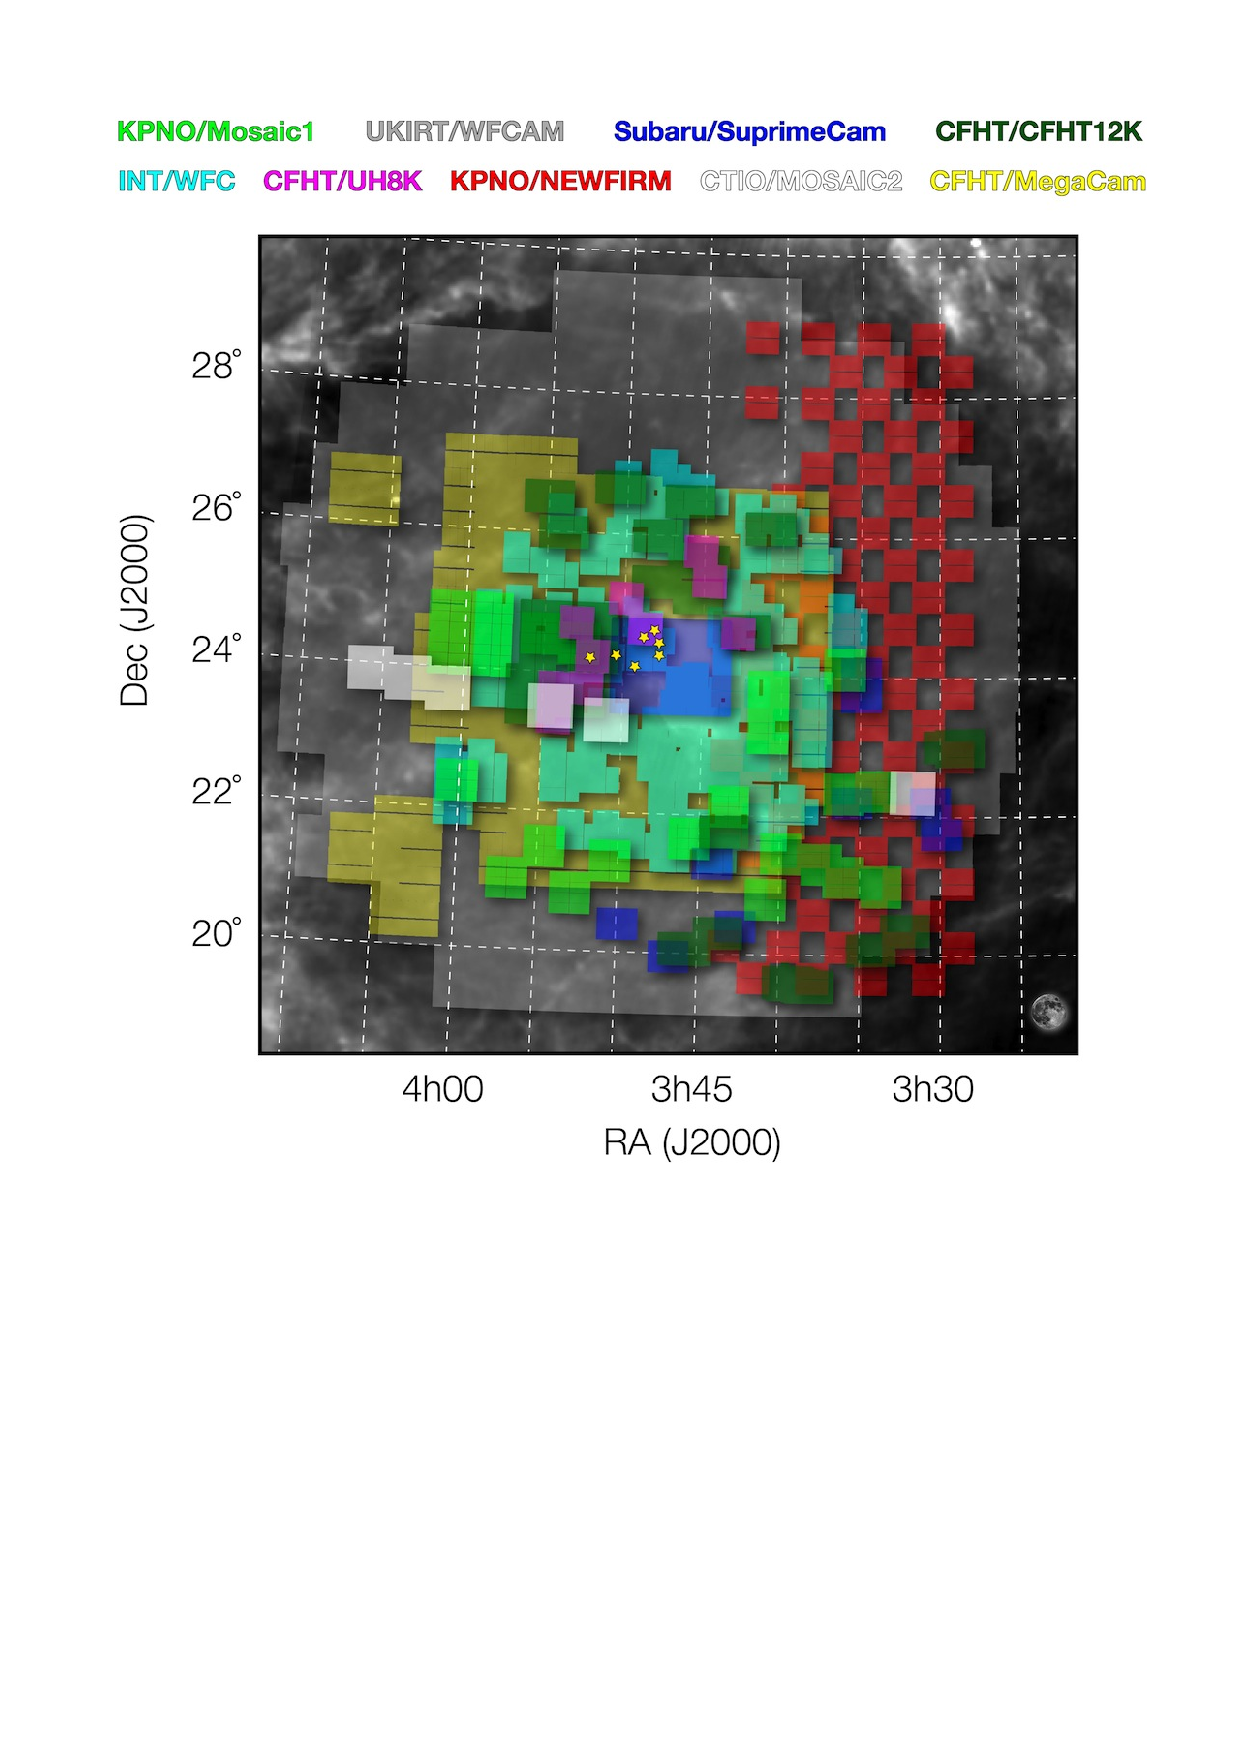
\includegraphics[width=\textwidth]{background/Figures/F1_Bouy2013.pdf}
\caption{Patchy composition of the Pleiades DANCe DR2. The moon shows the scale, and the yellow stars correspond to the central brightest objects of the Pleiades cluster. Reproduced from Figure 1 of \citet{Bouy2013},\textit{\usebibentry{Bouy2013}{title}}, \usebibentry{Bouy2013}{journal}, \usebibentry{Bouy2013}{volume}.}
\label{fig:originDANCeDR2}
\end{center}
\end{figure}

\begin{table}[htdp]
\caption{Summary of the Pleiades DANCe DR2.}
\begin{center}
\begin{tabular}{|c|c|c|c|c|c|c|c|}
\hline
Observable & Min. & 1st. Qu. & Median & Mean & 3rd. Qu. & Max. & NA's \\
\hline
\hline
RA [deg]&51.23 & 55.40 & 57.35 & 57.26 & 59.01 & 62.94 & 0\\
Dec. [deg] &19.12 &22.47 & 24.32 & 24.27  & 25.95 & 29.69 &0\\
$\mu_{\alpha} [mas\cdot yr^{-1}]$&-99.998& -6.060& -1.645& -1.240&3.401&99.996&0\\
$\mu_{\delta} [mas\cdot yr^{-1}]$&-99.997& -2.835&  2.548&  1.976&  7.017&99.989&0\\
u [mag]&13.6&20.4 &22.0 &21.6&23.3&25.2&1756374\\
g [mag]& 9.4   &19.6   &22.1   &21.1   &23.3   &25.5 &1492564\\
r [mag] &  8.4  &17.6   &21.3   &20.3   &22.6   &25.1   &1222853\\
i [mag] &  7.5  &20.0  &21.6  &21.0  &22.7  &25.5  &820861\\
z [mag]&11.2  &17.9  &19.3  &18.9  &20.2  &25.0  &697412\\
Y [mag]& 8.3  &17.2  &18.5  &18.1  &19.4  &24.2  &688144\\
J [mag]& 2.8  &16.7  &17.9  &17.5  &18.8  &23.1  &645469\\
H [mag]& 2.0  &16.1  &17.3  &16.9  &18.1  &20.9  &653682\\
$K_s$ [mag]& 1.8 &16.0&  17.0  &16.7  &17.7  &23.8  &561745\\
\hline
\end{tabular}
\end{center}
\label{tab:DR2properties}
\end{table}%

\begin{table}[ht!]
\caption{Uncertainties of the Pleiades DANCe DR2.}
\begin{center}
\begin{tabular}{|c|c|c|c|c|c|c|c|}
\hline
Observable & Min. & 1st. Qu. & Median & 3rd. Qu. & Max. &Mean\\
\hline
\hline
RA [deg]&8.900e-08 &9.270e-07&1.933e-06&4.037e-06&2.156e-02&3.173e-06\\
Dec. [deg] &8.900e-08&9.270e-07&1.932e-06&4.037e-06&2.156e-02&3.173e-06\\
$\mu_{\alpha} [mas\cdot yr^{-1}]$&2.01e-01 &1.89e+00& 4.35e+00& 1.00e+01& 1.49e+22&3.99e+16\\ 
$\mu_{\delta} [mas\cdot yr^{-1}]$&1.92e-01 &1.89e+00 &4.35e+00 &1.00e+01 & 4.71e+09&1.42e+04\\
u [mag] &3.73e-04& 8.07e-03& 3.06e-02& 8.56e-02& 2.17e-01&5.48e-02\\
g [mag] &1.72e-01 & 1.02e-02&  3.90e-02 & 7.90e-02 & 1.82e+00&5.34e-02\\
r [mag] & 2.83e-04 & 1.54e-02& 4.88e-02 &1.04e-01& 1.42e+00&6.34e-02\\
i [mag] & 4.04e-04 & 9.03e-03&  2.73e-02& 5.85e-02& 2.40e+00&4.37e-02\\
z [mag] & 6.49e-04& 5.62e-02& 9.16e-02& 1.85e-01& 3.12e+00&1.34e-01\\
Y [mag] & 3.00e-02& 5.21e-02& 6.50e-02& 1.03e-01& 9.01e+00&8.56e-02\\
J [mag] & 1.60e-02& 5.24e-02& 6.66e-02& 1.04e-01& 8.89e+00&8.57e-02\\
H [mag] & 1.40e-02& 5.28e-02& 7.04e-02& 1.10e-01& 1.00e+01&8.85e-02\\
$K_s$[mag]&1.40e-02& 5.75e-02& 8.17e-02& 1.32e-01& 3.88e+01&1.04e-01\\
\hline
\end{tabular}
\end{center}
\label{tab:DR2uncertainties}
\end{table}%

\begin{figure}[ht!]
\begin{center}
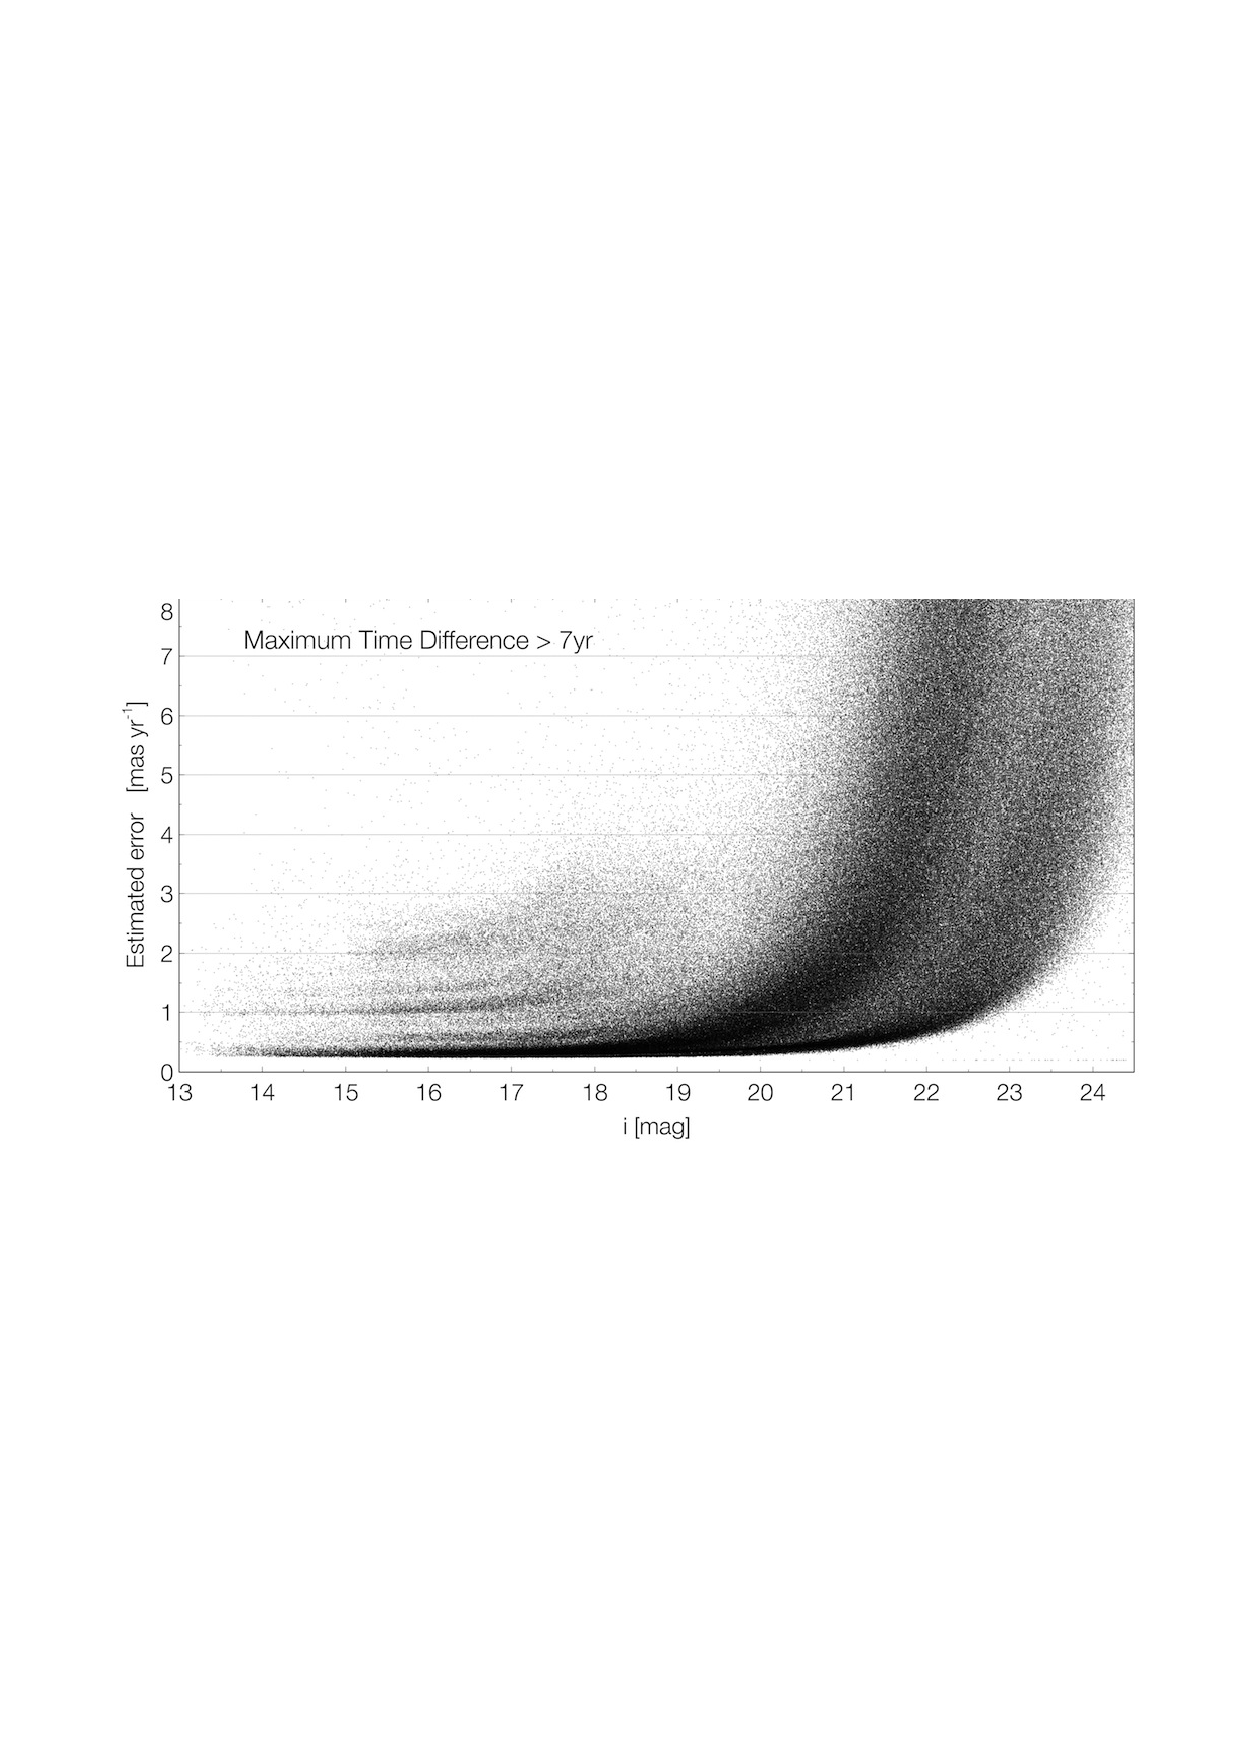
\includegraphics[height=8cm]{background/Figures/F12_Bouy2013.pdf}
\caption{Proper motion uncertainty as a function of the photometric magnitude in the $i$ band.Reproduced from Figure 12 of \citet{Bouy2013},\textit{\usebibentry{Bouy2013}{title}}, \usebibentry{Bouy2013}{journal}, \usebibentry{Bouy2013}{volume}.}
\label{fig:pmuncert}
\end{center}
\end{figure}

\subsection{Selection of observables}
\sloppy
As mentioned earlier, the Pleiades DANCe DR2 contains the positions $R.A.$,$Dec.$, proper motions, $\mu_{R.A.},\mu_{Dec.}$, and photometric $ugrizYJHK_s$ bands, of almost 2 million sources on the vicinity of the Pleiades clusters. Although these 13 observables carry information valuable to discriminate cluster members from field objects, not all of them discriminate in the same amount. \citet{Sarro2014} used important analysis with random forest to select the observables that were the most discriminants. They obtain that the AM, RF-2, and RF-3 reference sets containing the observables $\mu_{R.A.},\mu_{Dec.}$ proper motions, and photometric bands $rizYJHK_s$ were the most discriminants. However, these authors later excluded the $r$ band because most of objects in their training set do not have this band. Since most of the missing values in the $r$ band occur at the faint end, their resulting training set was bised towards the bright end. In a subsequent analysis using roughly the same methodology, \citet{Bouy2015} worked only the RF-2, which excludes also the $z$ band.

In this work I select the $\mu_{\alpha},\mu_{\delta},i,Y,J,H,K_s$ observables as my reference set, because these were the ones used \citet{Bouy2015}. This selection aims to compare our results with the previous ones of \citet{Sarro2014}, and \citet{Bouy2015}. However, for the analysis of the spatial distribution we later added the stellar positions ($R.A., Dec.$).

As will be described in Section \ref{subsect:cluster}, the photometry is modelled by parametric series of cubic splines. I choose the \emph{true} colour index $i-K_s$ (in the following $CI$) to be the parameter of these series. This colour allows the most one-to-one dependent-independent variable relation. This one-to-one relation can be seen in Figures \ref{fig:CI} and \ref{fig:otherCI}, where I show the colour-magnitude diagram of $K$ vs $i-K_s$ and $K$ vs colours $Y-K_s$, $J-K_s$, $H-K_s$, and $Y-J$, respectively.  This one-to-one relation is crucial to avoid degeneracies. Without it, two magnitudes could be described by the same colour index. Therefore a monotonic relation would not be valid. 

Thus, our photometric set of observables is made of $i-K_s, Y,J,H$ and $K_s$. 

\begin{figure}[htbp]
\begin{center}
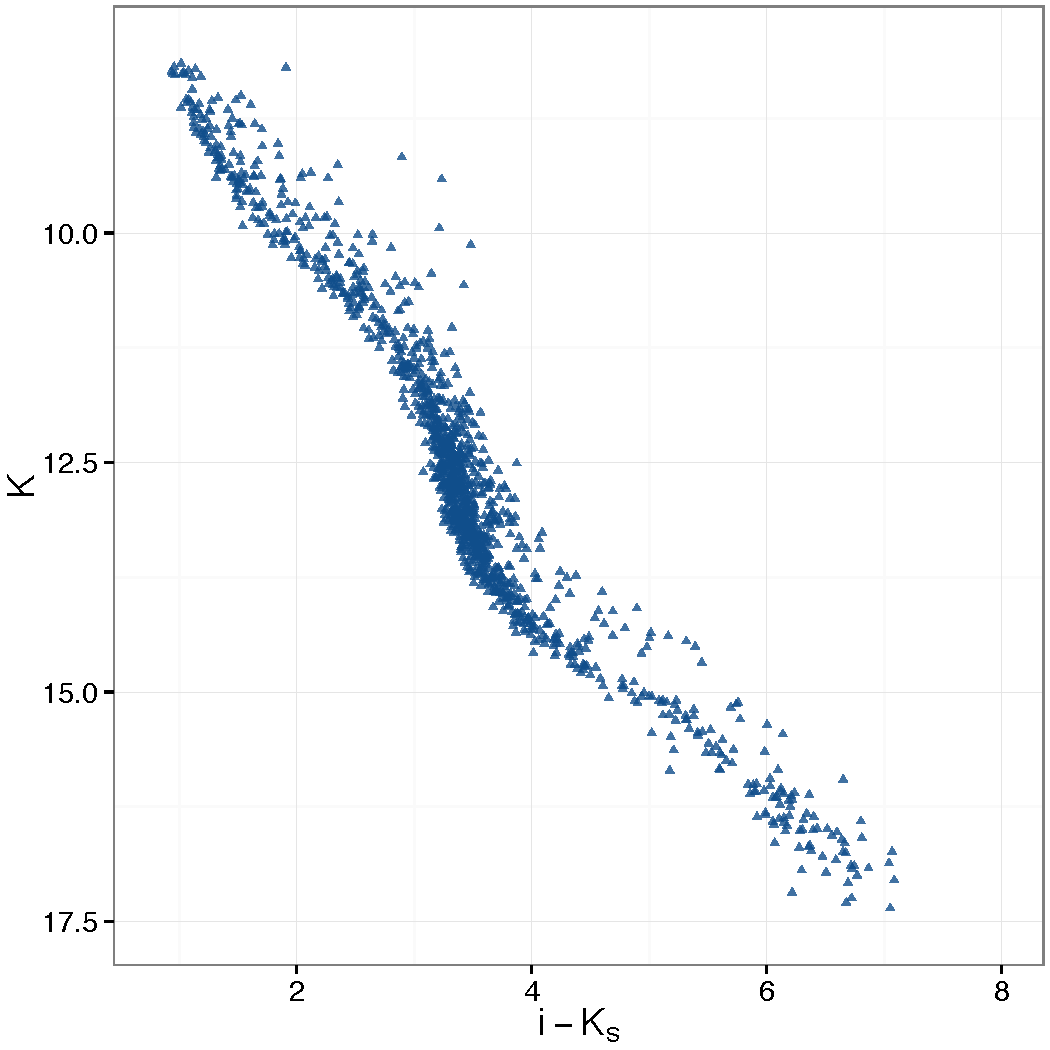
\includegraphics[page=1,height=8cm]{background/Figures/CIs.pdf}
\caption{$K_s$ vs $i-K_s$ CMD for the Pleiades candidate members of \citet{Bouy2015}}.
\label{fig:CI}
\end{center}
\end{figure}

\begin{figure}[ht!]
    \centering
    \begin{subfigure}[t]{0.45\textwidth}
        \includegraphics[page=2,height=6cm]{background/Figures/CIs.pdf}
        \caption{}
        \label{}
    \end{subfigure}
    \begin{subfigure}[t]{0.45\textwidth}
      \includegraphics[page=3,height=6cm]{background/Figures/CIs.pdf}
        \caption{}
        \label{} 
    \end{subfigure}
     \begin{subfigure}[t]{0.45\textwidth}
      \includegraphics[page=4,height=6cm]{background/Figures/CIs.pdf}
        \caption{}
        \label{} 
    \end{subfigure}
     \begin{subfigure}[t]{0.45\textwidth}
      \includegraphics[page=5,height=6cm]{background/Figures/CIs.pdf}
        \caption{}
        \label{} 
    \end{subfigure}
    \caption{CMD for the Pleiades candidate members of \citet{Bouy2015}. The magnitude $K_s$ is shown versus the colour indices: $Y-K_s$(a), $J-K_s$(b), $H-K_s$(c), and $Y-J$ (d).}
    \label{fig:otherCI}
\end{figure}


\subsection{Data preprocessing}
\label{sect:RDR2}
Since both photometry and proper motions carry crucial information for the disentanglement of the cluster population, we restrict the data set to only those objects with observed proper motions, and also at least two photometric entries in our photometric set ($i-K_s,Y,J,H,K_s$). These restrictions exclude 22 candidate members of \citet{Bouy2015}. Unfortunately, these objects have only one observed value in the photometry. For these particular objects, we compute their marginal proper motion membership probability a posteriori, once the parameters of the model were inferred. The mode and 16 and 84 percentiles of their membership probabilities are listed in Table \ref{tab:22excluded}. Only four of these 22 objects have membership probabilities below 0.5, which may indicate they are contaminants. Since these membership probabilities were computed using only the kinematic information, these four members could not be discarded as probable candidate members.

\begin{table}[htdp]
\caption{Membership probabilities of the 22 excluded candidate members of \citet{Bouy2015}.}
\begin{center}
\begin{tabular}{|c|c|c|c|}
\hline
ID DANCe & $P_{16}$ & Mode & $P_{84}$\\
\hline
\hline
J035106.55+211604.3 &0.751182& 0.7774335&    0.785560\\
J035057.42+240630.8 &0.792295& 0.8090186&   0.829541 \\
J034704.76+252249.8& 0.701193& 0.7319624 &   0.750745\\
J034725.80+250832.7 &0.789872& 0.8169538 &  0.827954 \\
J034437.44+250815.6 &0.762013& 0.7773114 &   0.798125\\
J035125.88+244738.6& 0.883488& 0.9007972 &  0.905823 \\
J034235.64+215029.7 &0.838538& 0.8662402 &  0.871439 \\
J034516.66+243432.1 &0.862284& 0.8666611 &   0.881004\\
J034926.12+235714.8& 0.852537& 0.8606685 &  0.866286 \\
J034920.60+244635.9 &0.923319& 0.9270399 &  0.935532 \\
J035300.63+233252.3 &0.762996& 0.7747163 &  0.781901 \\
J034606.52+235020.2& 0.928688& 0.9333306 &  0.940772 \\
J035040.89+245657.7 &0.509435& 0.5215143 &  0.530379 \\
J034845.33+233124.8 &0.260551& 0.2650812 &  0.275513 \\
J034713.67+234953.3& 0.814689& 0.8489593 &  0.855902 \\
J034546.48+234743.0 &0.897035& 0.9098442 &  0.912059 \\
J034548.95+235110.2 &0.933892& 0.9376429 &   0.945558\\
J035202.26+242148.1& 0.248011& 0.2649874 &   0.305949\\
J035313.22+235540.8 &0.518388& 0.5425345 &  0.553376 \\
J034425.60+244052.5 &0.581242& 0.5902633 &  0.602096 \\
J035518.38+245637.2& 0.198074& 0.2087989 &  0.252831 \\
J035418.93+252944.0& 0.366009& 0.3760922 &  0.386213 \\
\hline
\end{tabular}
\end{center}
\label{tab:22excluded}
\end{table}%


Furthermore, we restrict the lower limit of the $CI$ to the value of the brightest cluster member, $CI =0.8$. We do not expect to find new bluer members in the bright part of the CMDs. Also, we set the upper limit of the CI at one magnitude above the colour index of the reddest known cluster member, $CI=8$, thus allowing for new discoveries. Due to the sensitivity limits of the DR2 survey in $i$ and $K_s$ bands,\cite[$i\approx23$ mag and $K_s\approx18$ mag, see Appendix A of][]{Bouy2015}, objects with $CI>8$ have $K_s$ magnitudes $\geq 16$ mag. This combination of CI and $K_s$ magnitude is incompatible with the cluster sequence. Thus, we discard a priori these 695 objects as cluster members. With the previous restrictions to the DANCe DR2, it was reduced to 1 424 893 objects.

%In recent days, our research group has developed a GPU version of the methodology that I present here. This version is ten times faster than the old CPU one that I developed throughout my research. However, here I present the results obtained using the CPU version, the fastest one available at that moment.

Our computational constraints and the costly computations of our methodology (see Sect. \ref{sect:BHM}), prevented its application to the entire data set. However, since the precision of our methodology, as that of any statistical analysis, increases with the number of independent observations, we find that a size of $10^5$ source for our data is a reasonable compromise. Although a smaller data set produces faster results, it also renders a less precise and potentially more biased model of the field (in the area around the cluster) and therefore, a more contaminated model of the cluster. Thus, our data set was restricted to the $10^5$ objects with highest membership probabilities according to \citet{Bouy2015}. In the following I refer to this data set as the restricted DR2 or RDR2. The majority of these objects ($\approx$98\%) belong to the field with cluster membership probabilities about zero, according to \citet{Sarro2014,Bouy2015}. Thus, under the assumption that the membership probabilities given by these authors are correct, the probability of leaving out a cluster member is negligible. For the remaining of the objects in the Pleiades DANCe DR2, we assign membership probabilities \emph{a posteriori}, once the cluster model is constructed. 



